\documentclass[conference]{IEEEtran}

\usepackage{cite}
\usepackage{amsmath,amssymb,amsfonts}
\usepackage{graphicx}
\usepackage{textcomp}
\usepackage{xcolor}
\usepackage{booktabs}
\usepackage{url}
\usepackage{float}
\usepackage{placeins}

\graphicspath{{figures/}}

% Allow more floats per page and reduce minimum text fraction
\renewcommand{\topfraction}{0.9}
\renewcommand{\bottomfraction}{0.8}
\renewcommand{\textfraction}{0.07}
\renewcommand{\floatpagefraction}{0.85}
\setcounter{topnumber}{4}
\setcounter{bottomnumber}{2}
\setcounter{totalnumber}{6}

\begin{document}

\title{Biomedical Text Embeddings Weakly Capture Chromatin Accessibility
Similarity: A Large-Scale Measurement Study}

\author{}

\maketitle

\begin{abstract}
The extent to which biomedical text metadata can serve as a proxy for
chromatin accessibility similarity remains unknown. We conducted a systematic
measurement study comparing pairwise cosine similarity matrices across
12 distinct embedding types (Atacformer,
regulatory potential (RP), four biomedical language models tested in
full-metadata and cell-type-name-only configurations, term
frequency-inverse document frequency (TF-IDF), and a
random Gaussian baseline) across 32,245 human assay for transposase-accessible
chromatin with sequencing (ATAC-seq) experiments from
ChIP-Atlas. Using Spearman rank
correlation, Mantel permutation tests, and top-$k$ neighborhood overlap, we
find that apparent text--chromatin agreement is driven largely by experiments
with few called peaks. These experiments retain mainly promoter peaks (median
69 to 75\% within 1~kb of a transcription start site) and therefore resemble one
another in both chromatin representations regardless of cell type. On the full
dataset, text embeddings correlate with Atacformer similarity at $r = 0.20$ to
$0.28$, but among the 17,232 well-covered experiments ($\geq$5,000 peaks) this
falls to $r = 0.011$ to $0.016$, with less than 0.1\% shared nearest neighbors.
Text embeddings instead show weak but consistent agreement with RP
($r = 0.06$ to $0.10$; 31 to 35\% of top-5 neighbors shared), reflecting the
coarse cell-type structure that both encode. Sample titles, which encode data
provenance rather than biology, carry most of the full-dataset text signal.
TF-IDF matches all large language models (LLMs) in well-covered experiments,
indicating that semantic understanding adds little beyond surface-level
vocabulary. These results bound the utility of text metadata as a proxy for
chromatin similarity and show that peak count must be controlled when
comparing chromatin representations across public repositories.
\end{abstract}

\begin{IEEEkeywords}
genomics, bioinformatics, chromatin, natural language processing,
transformers, feature extraction, correlation, similarity measures
\end{IEEEkeywords}


% ── Introduction ──────────────────────────────────────────────────────────────
\section{Introduction}

The rapid growth of epigenomics databases such as ChIP-Atlas~\cite{chipatlas},
Encyclopedia of DNA Elements (ENCODE)~\cite{encode}, and Roadmap Epigenomics~\cite{roadmap} has produced tens
of thousands of ATAC-seq experiments across diverse human cell types and
conditions. Organizing, retrieving, and comparing these experiments requires
similarity measures that reflect the underlying biology. A natural question
arises: to what extent can text metadata associated with experiments (cell
type labels, experimental descriptions, and publication titles) serve as a
proxy for chromatin accessibility similarity?

This question has direct practical implications. If text embeddings of experimental
metadata closely approximate chromatin-based similarity measures (such as those
derived from Atacformer or RP), they could enable natural-language
retrieval and annotation of ATAC-seq data without access to the raw signal,
potentially democratizing the use of large epigenomics repositories.
If agreement is limited, the results instead point to fundamental limits on
what text can capture and motivate investment in chromatin-specific
representation learning.

Recent advances in biomedical natural language processing have produced
powerful text encoders pretrained on large biomedical corpora.
PubMedBERT~\cite{pubmedbert} is pretrained from scratch on PubMed abstracts
and full-text articles. SapBERT~\cite{sapbert} and MedCPT~\cite{medcpt} are
both initialized from a pretrained PubMedBERT checkpoint and further
fine-tuned for different objectives: SapBERT via self-alignment on Unified Medical Language System (UMLS)
synonym pairs, and MedCPT via contrastive learning on PubMed search logs.
These models achieve strong performance on biomedical entity recognition,
relation extraction, and information retrieval, yet whether their semantic
representations capture the biological relationships encoded in chromatin
accessibility data has not been systematically evaluated.

Atacformer~\cite{atacformer} is a transformer trained on ATAC-seq data using
triplet margin loss to produce experiment-level embeddings that cluster by cell
type and chromatin state. Regulatory potential (RP)~\cite{lisa2} provides a
complementary, functional-genomics-derived signal: a gene-activation-weighted
summary of chromatin accessibility indexed by gene transcription start sites (TSS).

We compare pairwise cosine similarity matrices from 12 embedding types (chromatin
models, biomedical LLMs in full-metadata and name-only configurations, TF-IDF, and a random baseline) across 32,245 curated
human ATAC-seq experiments, treating both agreement and disagreement as
informative findings. Because public repositories mix experiments of very
different quality, we also examine how the number of called peaks shapes
these comparisons, and base our primary analysis on well-covered experiments.

The key findings are:
\begin{itemize}
  \setlength{\itemsep}{0pt}
  \setlength{\parsep}{0pt}
  \setlength{\topsep}{0pt}
  \item Peak count dominates similarity in both chromatin representations;
        low-peak experiments, which retain mainly promoter peaks, inflate
        apparent text--chromatin agreement on the full dataset.
  \item In well-covered experiments, text does not track Atacformer
        similarity and tracks RP only weakly, capturing coarse cell-type
        identity rather than fine-grained chromatin variation.
  \item Vocabulary overlap alone (TF-IDF) matches all biomedical LLMs, and
        sample titles, which encode data provenance, carry most of the
        full-dataset text signal.
\end{itemize}

% ── Methods ───────────────────────────────────────────────────────────────────
\newpage
\section{Methods}

Fig.~\ref{fig:schematic} summarizes the overall study design: chromatin-based
embeddings (Atacformer, RP) and text-based embeddings (biomedical and general
language models, TF-IDF, random) are computed for each experiment, converted
into pairwise similarity matrices at two levels of aggregation, and compared
using the four metrics described in Section~\ref{sec:metrics}.

\begin{figure*}[!t]
  \centering
  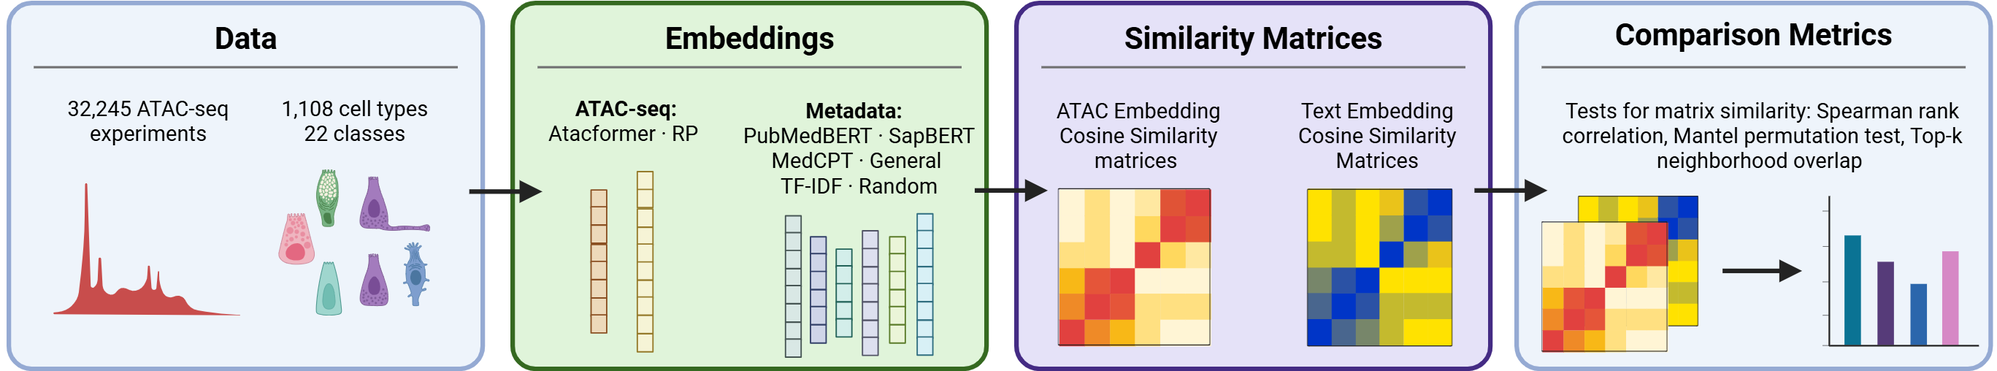
\includegraphics[width=\linewidth]{fig1.png}
  \caption{Study design. ATAC-seq experiments are embedded
  using chromatin-based models (Atacformer, RP), text encoders (biomedical and
  general language models, TF-IDF), and a random baseline. Pairwise cosine
  similarity matrices are computed at cell-type-aggregated and full-dataset
  levels and compared using four complementary metrics.
  Created with BioRender.com~\cite{biorender}.}
  \label{fig:schematic}
\end{figure*}

\subsection{Dataset}

We obtained 48,822 human ATAC-seq experiments from ChIP-Atlas
(hg38 assembly)~\cite{chipatlas}. We removed 16,567 experiments with
corrupted or empty BED files and 10 experiments producing zero regulatory
potential signal near gene TSSs, yielding a curated set of 32,245
experiments spanning 1,108 cell types.

ChIP-Atlas peak sets are called at a stringent threshold
($q < 10^{-10}$), and the number of peaks per experiment varies over more than
three orders of magnitude (median 6,287; interquartile range 780--19,836;
8,964 experiments have fewer than 1,000 peaks). Because experiments with few
peaks retain mainly the strongest, largely constitutive sites
(Section~\ref{sec:coverage}), our primary analysis uses the 17,232
experiments with at least 5,000 peaks (hereafter \textit{well-covered}
experiments). We report results on all 32,245 experiments as a contrast.

\subsection{Atacformer Embeddings}
\label{sec:atacformer}

We encoded each experiment using \url{databio/atacformer-base-hg38}
(AtacformerForCellClustering)~\cite{atacformer}, a transformer trained with
triplet margin loss. Peak BED files were tokenized using the gtars Tokenizer
with a vocabulary of 890K genomic regions. Up to 1,024 randomly sampled peak
tokens were mean-pooled to produce a 192-dimensional embedding per experiment.

\subsection{Regulatory Potential Embeddings}

We computed RP for each experiment using a LISA2-style exponential decay
model~\cite{lisa2}: each chromatin peak's contribution to a given gene is
weighted by $w(d) = e^{-d/10\,\text{kb}}$, where $d$ is the distance to
the gene's TSS, with peaks overlapping annotated exons assigned a fixed weight
of 1.0 (replacing the exponential decay for those peaks).
Summing across all peaks yields a per-gene RP score; stacking over all hg38
autosomal gene TSSs maps each experiment to a 40,772-dimensional vector.

\subsection{Text Embeddings}
\label{sec:text_emb}

This section describes text- and metadata-based embedding methods only;
chromatin-based embeddings (Atacformer and RP) are described in the two
preceding subsections.

For each experiment we constructed a full metadata string by concatenating
available fields: \{cell\_type\}. \{cell\_type\_class\}.
\{cell\_type\_description\}. \{title\}. We embedded this string using four
encoders, all of which produce 768-dimensional embeddings:
PubMedBERT~\cite{pubmedbert}
(\url{microsoft/BiomedNLP-BiomedBERT-base-uncased-abstract-fulltext}, mean
pooling), SapBERT~\cite{sapbert}
(\url{cambridgeltl/SapBERT-from-PubMedBERT-fulltext}, classification token (CLS) pooling),
MedCPT~\cite{medcpt} (\url{ncbi/MedCPT-Query-Encoder}, mean
pooling), and a General encoder~\cite{mpnet}
(\url{sentence-transformers/all-mpnet-base-v2}, mean pooling). To isolate
the contribution of cell type identity, we also encoded each experiment using
only the cell type name string with all four models (cell-type-name-only
ablation). We additionally computed TF-IDF embeddings (top 2,048
features, sublinear TF, 2,048-dimensional) and a random Gaussian
baseline (192-dimensional, seed 42).

\subsection{Similarity Matrices and Comparison Metrics}
\label{sec:metrics}

For each embedding type we constructed pairwise cosine similarity matrices at
two levels of aggregation.

\textit{Cell-type-aggregated level.} Individual experiment embeddings were
mean-pooled within each cell type to produce one representative vector per cell
type. A corpus mean vector was computed as the arithmetic mean over up to
10,000 randomly sampled individual experiment embeddings and subtracted from
each cell-type mean vector. For every pair of cell types $(i, j)$, the cosine
similarity between their centered vectors was computed and stored in entry
$(i, j)$ of the matrix, yielding a symmetric $1{,}108 \times 1{,}108$ matrix
with ones on the diagonal.

\textit{Full-dataset level.} The same corpus-centering procedure was applied to
all 32,245 individual experiment embeddings. For every pair of experiments
$(i, j)$, the cosine similarity between their centered embedding vectors was
computed and stored in entry $(i, j)$, yielding a symmetric
$32{,}245 \times 32{,}245$ matrix with ones on the diagonal.

Corpus centering corrects for anisotropy in transformer mean-pool
representations: without it, embeddings tend to cluster in a narrow cone in
the embedding space, which inflates cosine similarities uniformly and obscures
relative differences in pairwise structure. The centering vector was estimated
from individual experiments (not from cell-type means) to avoid conflating
aggregation level with the centering baseline.

We quantified agreement between each text-embedding similarity matrix and each
chromatin reference (Atacformer and RP) using four metrics:
\begin{enumerate}
  \item Spearman rank correlation ($r$) on upper-triangle edge weights.
  \item Mantel permutation test (1,000 permutations) for empirical
        $p$-values at the cell-type level.
  \item Bootstrap confidence intervals for $r$ (1,000 resamples
        of cell types/experiments, with 50,000 randomly sampled pairs per
        resample), reported at both the cell-type and full-dataset scale as a
        scale-independent measure of effect-size precision.
  \item Top-$k$ neighborhood overlap: mean fraction of shared top-$k$
        nearest neighbors, $k \in \{5, 10, 20, 50\}$.
\end{enumerate}

All analyses were conducted with both Atacformer and RP as reference
structures (i.e., the chromatin similarity structures against which
text-based embeddings are evaluated). For the primary (well-covered)
analysis, cell-type mean vectors were recomputed from well-covered
experiments only, and experiment-level matrices were restricted to the
17,232 well-covered experiments; the corpus mean used for centering was
unchanged. Full-scale correlations were estimated on $2 \times 10^6$
randomly sampled pairs.

\subsection{Technical Covariates and Sensitivity Analyses}
\label{sec:tech_methods}

For each experiment we recorded the number of peaks in its ChIP-Atlas BED
file and the fraction of peaks whose midpoint lies within 1~kb of an
annotated RefSeq TSS (the same hg38 annotation used for RP). For a pair of
experiments we summarized peak count by \textit{depth match},
$-|\log_{10} n_i - \log_{10} n_j|$, and \textit{mean depth},
$(\log_{10} n_i + \log_{10} n_j)/2$. We used these quantities in four
analyses: (i) Spearman correlations computed within peak-count strata
(both experiments with $<$1K, 1--5K, 5--10K, or $\geq$10K peaks);
(ii) partial Spearman correlations controlling for depth match and mean depth
(and, separately, for same-cell-type and same-cell-type-class indicators),
computed by regressing covariate ranks out of each variable's ranks;
(iii) a title-only TF-IDF embedding (same settings as above, fit on the
\{title\} field alone) to isolate the contribution of sample titles; and
(iv) recomputation of all similarities without corpus centering. Uncertainty
for partial correlations was estimated by an experiment-level block
bootstrap (1,000 resamples of experiments, 200,000 pairs each).

\subsection{Decomposing LLM Signal from TF-IDF}

To determine whether LLMs encode biological information
beyond surface-level vocabulary overlap, we conducted three complementary
analyses comparing the full-text LLM embeddings against TF-IDF, both in
well-covered experiments and on the full 32,245-experiment dataset.

Pairwise similarity scatter. For each LLM, we sampled up to 25,000
random experiment pairs and plotted TF-IDF pairwise similarity against LLM
pairwise similarity, coloring each point by Atacformer similarity
(Fig.~\ref{fig:s3a}). Points
above the diagonal indicate pairs where the LLM assigns higher similarity than
TF-IDF; points below indicate the reverse. The Spearman correlation between
TF-IDF and LLM similarity vectors was computed over the same sample.

Partial Spearman correlation. We computed the partial Spearman
rank correlation of each LLM similarity matrix with Atacformer, controlling
for TF-IDF:
\begin{equation}
  r_{LM,AC \mid TF} =
    \frac{r_{LM,AC} - r_{LM,TF}\,r_{AC,TF}}
         {\sqrt{(1-r_{LM,TF}^{2})(1-r_{AC,TF}^{2})}}
\end{equation}
where $r_{X,Y}$ denotes the Spearman correlation of the upper-triangle
edge weights of matrices $X$ and $Y$. At the full scale, correlations were
estimated on a random subsample of $2 \times 10^6$ pairs from the
${\sim}520$M-element upper triangle. A positive partial correlation indicates
that the LLM encodes biological structure beyond vocabulary overlap; a value
near zero or negative indicates its Atacformer alignment is statistically
accounted for by TF-IDF (i.e., once TF-IDF's shared variance with Atacformer
is removed, the LLM contributes no additional association with chromatin similarity).

Cross top-$k$ neighborhood overlap. For each LLM and each
$k \in \{5, 10, 20, 50\}$, we computed the mean fraction of top-$k$ LLM
nearest neighbors that are also top-$k$ TF-IDF nearest neighbors, using the
same topk\_overlap procedure described above. High overlap indicates
the LLM's local structure recapitulates TF-IDF; low overlap indicates
genuinely distinct neighbor assignments.

% ── Results ───────────────────────────────────────────────────────────────────
\section{Results}

\subsection{Peak Count Inflates Apparent Text--Chromatin Agreement}
\label{sec:coverage}

Experiments with few peaks retain mainly promoter peaks. Below 10,000 peaks,
the median experiment has 69 to 75\% of its peaks within 1~kb of a TSS; this
falls to 39\% at 20,000--50,000 peaks and 24\% above 50,000
(Fig.~\ref{fig:coverage}a). Promoters of broadly expressed genes are accessible
in most cell types, so low-peak experiments resemble one another regardless of
cell type.

This shared promoter signal dominates the similarity structure of both
chromatin representations. Across all 32,245 experiments, Atacformer similarity
correlated with depth match (Section~\ref{sec:tech_methods}) at $r = 0.66$, and
RP similarity at $r = 0.59$, larger than any text--chromatin correlation we
observed. After controlling for depth match and mean depth, Atacformer--RP
agreement fell from $r = 0.215$ to $-0.018$. Across 406 cell types with
$\geq 10$ experiments, within-cell-type Atacformer similarity was strongly
predicted by the spread of peak counts within that cell type (Spearman
$\rho = -0.77$ with the SD of $\log_{10}$ peak count; RP: $\rho = -0.71$).

Text--Atacformer agreement on the full dataset is concentrated in these
low-peak experiments (Fig.~\ref{fig:coverage}b). When both experiments have
fewer than 1,000 peaks, text models correlate with Atacformer at
$r = 0.38$ to $0.41$; this falls to $0.08$--$0.09$ at 1,000--5,000 peaks,
$0.02$--$0.04$ at 5,000--10,000, and $0.007$--$0.012$ above 10,000.
Text--RP agreement shows the opposite trend, rising from $r = 0.04$--$0.10$
in the lowest stratum to $0.08$--$0.14$ in the highest
(Fig.~\ref{fig:coverage}c).

Within the metadata, sample titles carry most of the text signal. A TF-IDF
embedding of the title field alone correlated with Atacformer as strongly as
PubMedBERT on the full metadata string ($r = 0.275$ for both), and within a
cell type it exceeded every full-text model ($r = 0.24$ vs.\ $0.20$--$0.22$).
Controlling for title similarity reduced within-cell-type text--Atacformer
correlations to $r \approx 0.05$. ChIP-Atlas titles are SRA/GEO sample names
(e.g., ``Illumina HiSeq 2500 sequencing of SAMD00123421''), so this signal
reflects data provenance (study, platform, and naming conventions), which
covaries with library depth and quality, rather than biological content.
Cell-type labels themselves explained little of the full-data correlation:
controlling for same-cell-type and same-class indicators reduced PubMedBERT's
correlation with Atacformer only from $0.275$ to $0.254$.

The qualitative examples in Tables~\ref{tab:qual_atac} and~\ref{tab:qual_rp},
which pair experiments with high chromatin similarity but low text similarity,
illustrate the same artifact. All ten RP pairs consist of two low-peak
experiments ($\leq$1,438 peaks each, against a corpus median of 6,287), as
does the leading Atacformer pair (NCI-H1299 and CD4+ T cells; 1,181 and
1,272 peaks). We therefore base our primary analysis on well-covered
experiments ($\geq$5,000 peaks) and report full-dataset results as a contrast.
The 5,000-peak threshold is pragmatic: experiments with 5,000--10,000 peaks
remain promoter-rich (Fig.~\ref{fig:coverage}a), but experiment-level
correlations computed at a 10,000-peak threshold lead to the same conclusions.

\begin{figure*}[!t]
  \centering
  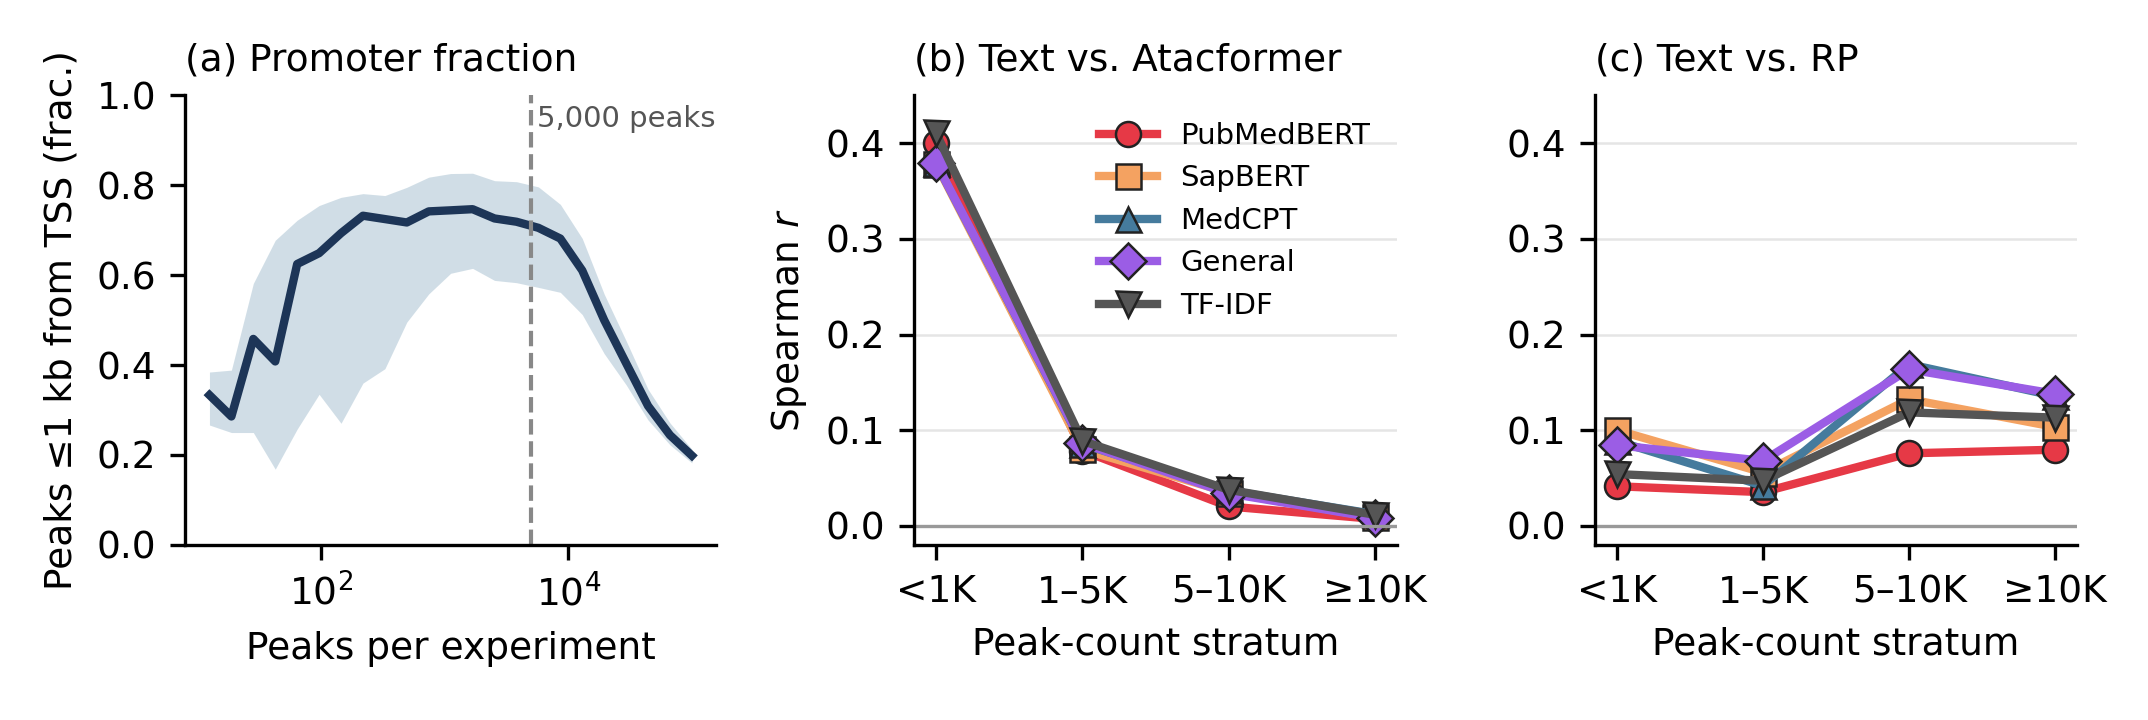
\includegraphics[width=\linewidth]{fig_coverage.png}
  \caption{Peak count and text--chromatin agreement. (a)~Fraction of each
  experiment's peaks within 1~kb of an annotated TSS vs.\ number of peaks
  (median and interquartile range in log-spaced bins; all 32,245 experiments).
  Dashed line: 5,000-peak threshold for the primary analysis. (b,c)~Spearman
  correlation of text-embedding similarity with Atacformer (b) and RP (c)
  similarity, computed separately for pairs in which both experiments fall in
  the same peak-count stratum (from $2 \times 10^6$ random pairs).}
  \label{fig:coverage}
\end{figure*}

\subsection{In Well-Covered Experiments, Text Tracks RP Weakly and Atacformer Not at All}

Sanity checks confirmed that Atacformer and RP cell-type means produce
coherent lineage structure, with immune, neural, and cancer cell types forming
distinct clusters, while text-based embeddings show coarser organization
(Fig.~\ref{fig:s1}).

\begin{figure*}[!t]
  \centering
  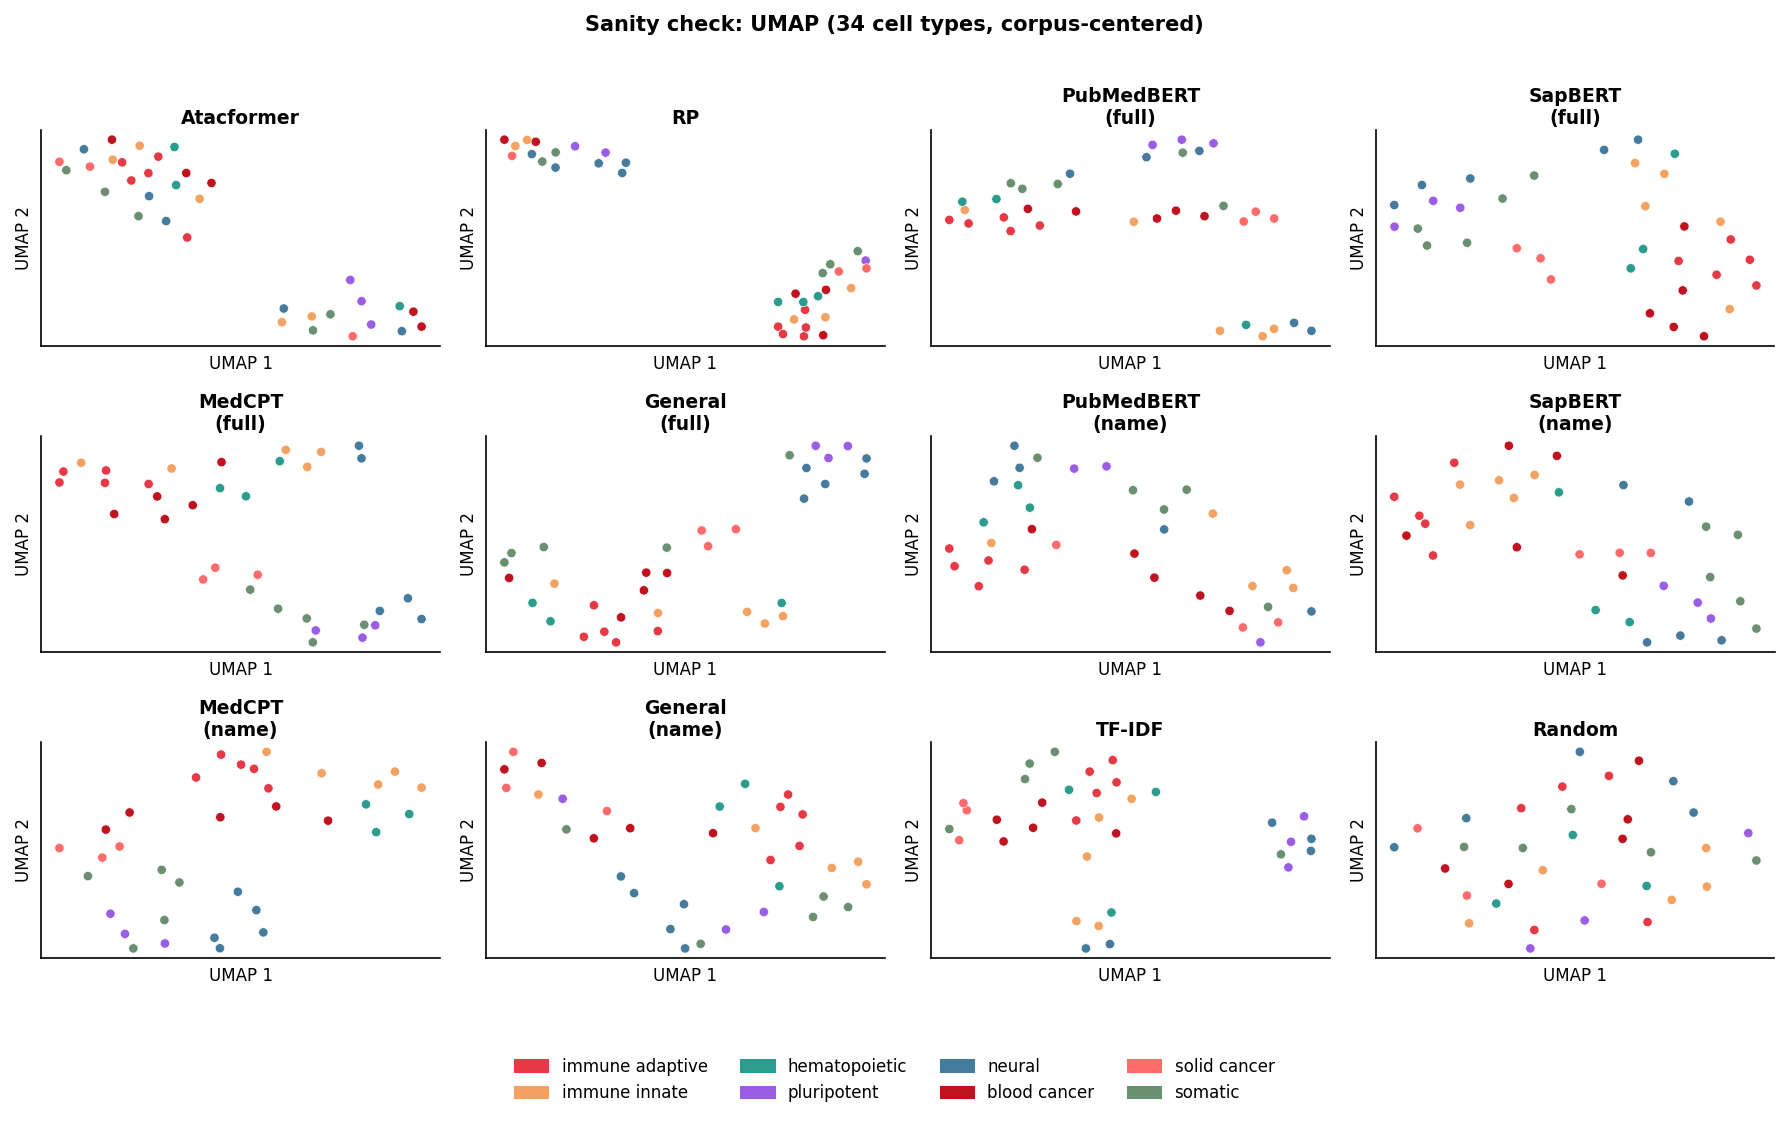
\includegraphics[width=\linewidth]{figS1a.png}
  \vspace{6pt}
  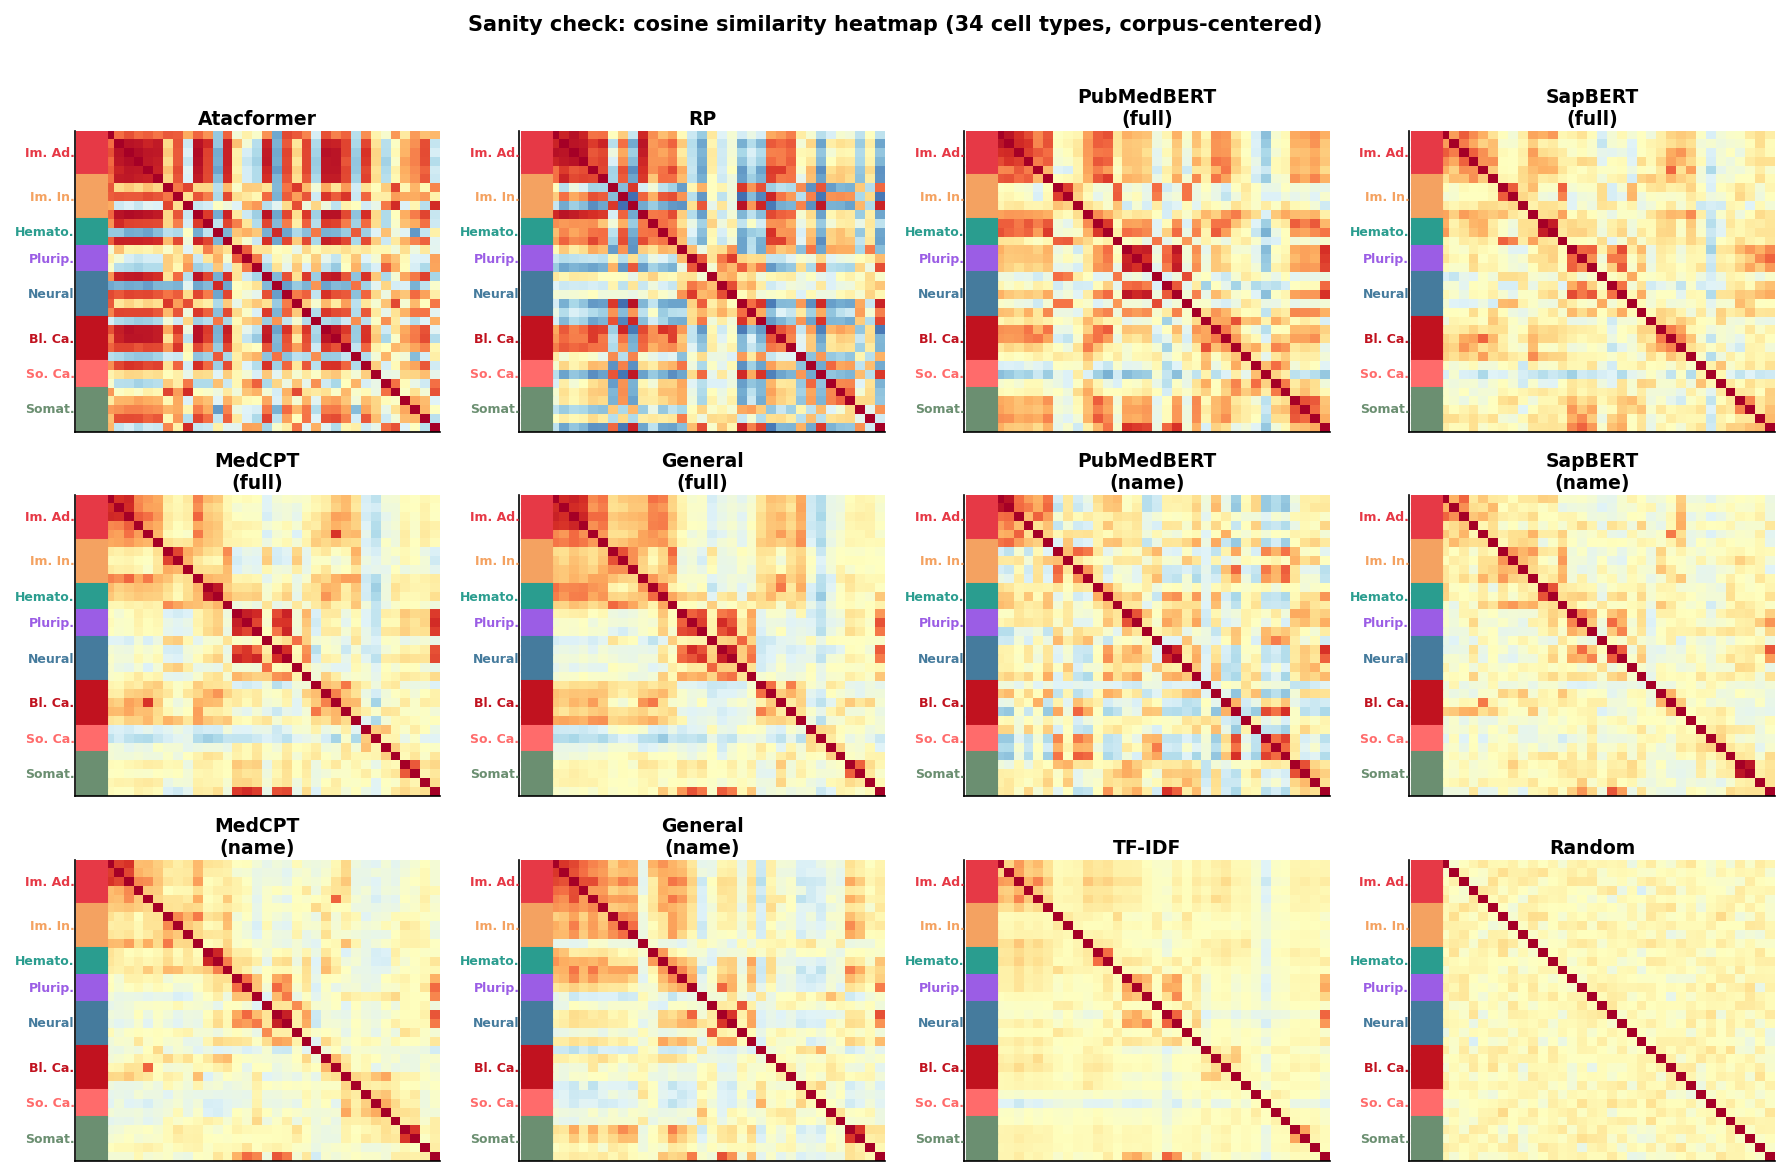
\includegraphics[width=\linewidth]{figS1b.png}
  \caption{Sanity check Uniform Manifold Approximation and Projection (UMAP) projections (top) and cosine
  similarity heatmaps (bottom) for all 12 embedding conditions over 34
  representative cell types manually selected to span major lineages (immune,
  neural, stem/progenitor, cancer, and stromal). Atacformer and RP show
  biologically coherent lineage clustering; text-based models show coarser,
  cell-type-level organization.}
  \label{fig:s1}
\end{figure*}

Among the 17,232 well-covered experiments (954 cell types), text embeddings
showed no positive agreement with Atacformer (Table~\ref{tab:spearman}). At
the cell-type-aggregated level, all full-text models and TF-IDF correlated
slightly negatively with Atacformer ($r = -0.074$ to $-0.023$; Mantel
$p > 0.98$). At the experiment level, correlations were indistinguishable from
zero in practical terms ($r = 0.011$ to $0.016$), compared with $r = 0.20$ to
$0.30$ on the full dataset. In contrast, all full-text models and TF-IDF
showed weak but consistent agreement with RP, both at the cell-type level
($r = 0.038$ to $0.068$; Mantel $p = 0.001$) and at the experiment level
($r = 0.061$ to $0.098$). Atacformer and RP agreed with each other at the
cell-type level ($r = 0.365$) but only modestly across experiments
($r = 0.107$).

Cell-type-name-only variants agreed with RP less than the full-text models at
the cell-type level ($r = 0.003$ to $0.021$), indicating that the description
and title fields contribute beyond the cell-type name; at the experiment level
they reached $r = 0.035$ to $0.080$.

\begin{table*}[!t]
  \centering\footnotesize
  \caption{Spearman rank correlation ($r$) of each embedding's similarity
  with Atacformer and RP similarity. Primary analysis: well-covered experiments
  ($\geq$5,000 peaks; 954 cell types, 17,232 experiments), with 95\%
  bootstrap confidence intervals at the experiment level (1,000 resamples of
  experiments, 50,000 pairs each). Contrast: all 32,245 experiments, as in the
  original analysis. Significance markers (one-sided Mantel permutation test,
  1,000 permutations) are reported at the cell-type level only.}
  \label{tab:spearman}
  \setlength{\tabcolsep}{4pt}
  \begin{tabular}{l ccc ccc}
    \toprule
    & \multicolumn{3}{c}{vs.\ Atacformer} & \multicolumn{3}{c}{vs.\ RP} \\
    \cmidrule(lr){2-4} \cmidrule(lr){5-7}
    & \multicolumn{2}{c}{$\geq$5,000 peaks} & All & \multicolumn{2}{c}{$\geq$5,000 peaks} & All \\
    \cmidrule(lr){2-3} \cmidrule(lr){5-6}
    Embedding & Cell type & Experiment [95\% CI] & Experiment & Cell type & Experiment [95\% CI] & Experiment \\
    \midrule
    Atacformer / RP          & $0.365^{***}$ & $0.107$ [0.097, 0.116]  & $0.216$ & $0.365^{***}$ & $0.107$ [0.097, 0.117]  & $0.216$ \\
    PubMedBERT (full text)   & $-0.030^{ns}$ & $0.011$ [0.001, 0.021]  & $0.276$ & $0.038^{***}$ & $0.061$ [0.051, 0.072]  & $0.092$ \\
    SapBERT (full text)      & $-0.023^{ns}$ & $0.013$ [0.004, 0.022]  & $0.248$ & $0.067^{***}$ & $0.079$ [0.069, 0.088]  & $0.074$ \\
    MedCPT (full text)       & $-0.074^{ns}$ & $0.016$ [0.006, 0.025]  & $0.229$ & $0.062^{***}$ & $0.098$ [0.087, 0.107]  & $0.090$ \\
    General (full text)      & $-0.053^{ns}$ & $0.014$ [0.005, 0.023]  & $0.196$ & $0.068^{***}$ & $0.095$ [0.085, 0.104]  & $0.088$ \\
    TF-IDF                   & $-0.057^{ns}$ & $0.016$ [0.007, 0.026]  & $0.300$ & $0.065^{***}$ & $0.091$ [0.081, 0.101]  & $0.089$ \\
    PubMedBERT (name only)   & $-0.071^{ns}$ & $0.005$ [$-$0.004, 0.013] & $0.090$ & $0.003^{ns}$  & $0.035$ [0.027, 0.044]  & $0.018$ \\
    SapBERT (name only)      & $-0.101^{ns}$ & $0.008$ [$-$0.001, 0.017] & $0.137$ & $0.013^{ns}$  & $0.066$ [0.056, 0.074]  & $0.026$ \\
    MedCPT (name only)       & $-0.098^{ns}$ & $0.012$ [0.002, 0.020]  & $0.068$ & $0.021^{*}$   & $0.080$ [0.070, 0.089]  & $0.022$ \\
    General (name only)      & $-0.060^{ns}$ & $0.006$ [$-$0.003, 0.016] & $0.090$ & $0.015^{*}$   & $0.039$ [0.030, 0.048]  & $0.010$ \\
    Random Gaussian          & $0.003^{*}$   & $0.000$ [$-$0.008, 0.009] & $0.000$ & $0.003^{*}$   & $0.000$ [$-$0.009, 0.009] & $0.000$ \\
    \bottomrule
  \end{tabular}
  \\[3pt]
  {\footnotesize $^{***}p \leq 0.001$; $^{*}p < 0.05$; $^{ns}$ not significant. The marginal
  random-baseline result arises because subtracting the corpus mean gives cell-type means of
  large cell types a shared direction.}
\end{table*}

\subsection{Biomedical Language Models Add Little Beyond Vocabulary Overlap}
\label{sec:partial_corr}

In well-covered experiments, TF-IDF matched the LLMs against both references
(Table~\ref{tab:spearman}). Partial correlations with Atacformer after
controlling for TF-IDF were near zero for all four LLMs
($r_{\mathrm{partial}} = 0.000$ to $0.006$; bootstrap 95\% CIs within
$[-0.004, 0.011]$). Against RP, MedCPT, the general encoder, and SapBERT
retained small residual associations beyond TF-IDF
($r_{\mathrm{partial}} = 0.046$, $0.046$, and $0.037$), whereas PubMedBERT did
not ($0.003$). LLM and TF-IDF similarity structures were strongly correlated
($r = 0.52$ to $0.73$), and 44 to 45\% of each LLM's top-5 neighbors were
also TF-IDF neighbors.

On the full dataset (Figs.~\ref{fig:decomp}--\ref{fig:s3b}), PubMedBERT
($r_{\mathrm{partial}} = +0.051$; 95\% CI $[0.048, 0.059]$) and SapBERT
($+0.045$; $[0.039, 0.049]$) retained positive partial correlations with
Atacformer, whereas MedCPT ($-0.030$) and the general encoder ($-0.042$) did
not. This pattern is robust to experiment-level resampling but disappears in
well-covered experiments, and it depends on corpus centering: without
centering, all three biomedical models show large residuals (e.g.,
PubMedBERT $r_{\mathrm{partial}} = 0.257$), and PubMedBERT ($r = 0.292$)
rather than TF-IDF ($r = 0.153$) shows the highest raw correlation with
Atacformer. We therefore do not interpret the full-dataset differences among
LLMs as evidence about pretraining or fine-tuning objectives.

\begin{figure}[!t]
  \centering
  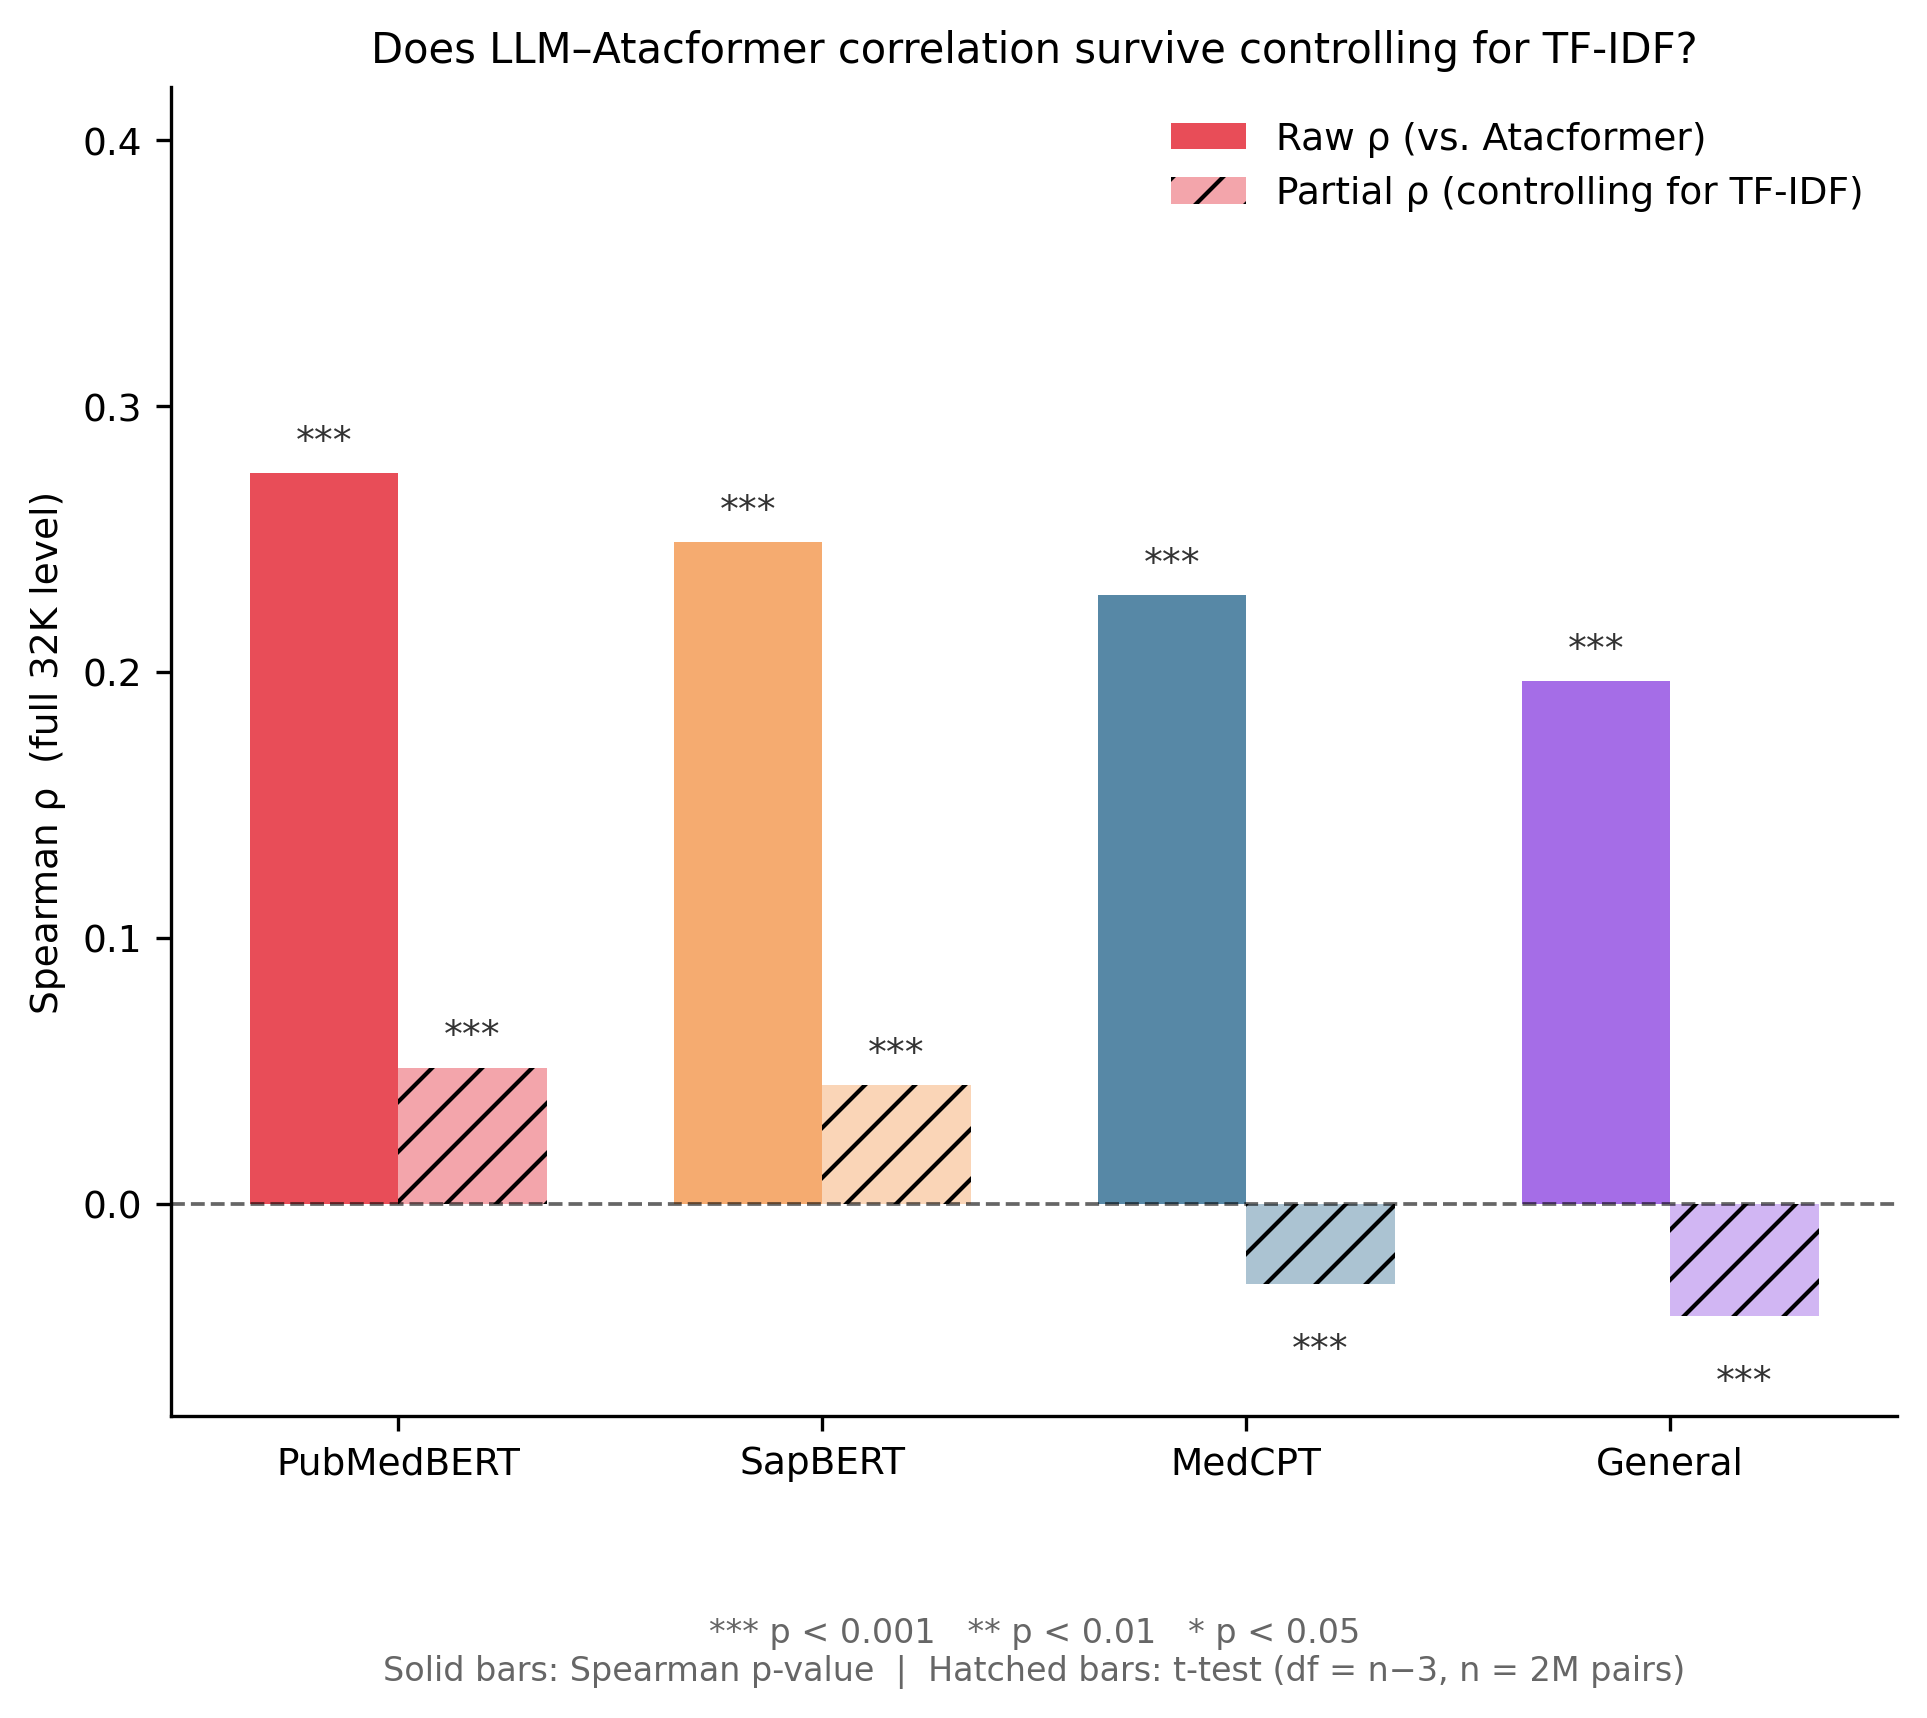
\includegraphics[width=\columnwidth]{fig4a.png}
  \caption{All 32,245 experiments (contrast analysis). Spearman $r$ vs.\
  Atacformer (solid bars) and partial Spearman $r_{\mathrm{partial}}$ after
  controlling for TF-IDF (hatched bars). In well-covered experiments, all
  partial correlations are $\leq 0.006$ (Section~\ref{sec:partial_corr}).}
  \label{fig:decomp}
\end{figure}

\begin{figure}[!t]
  \centering
  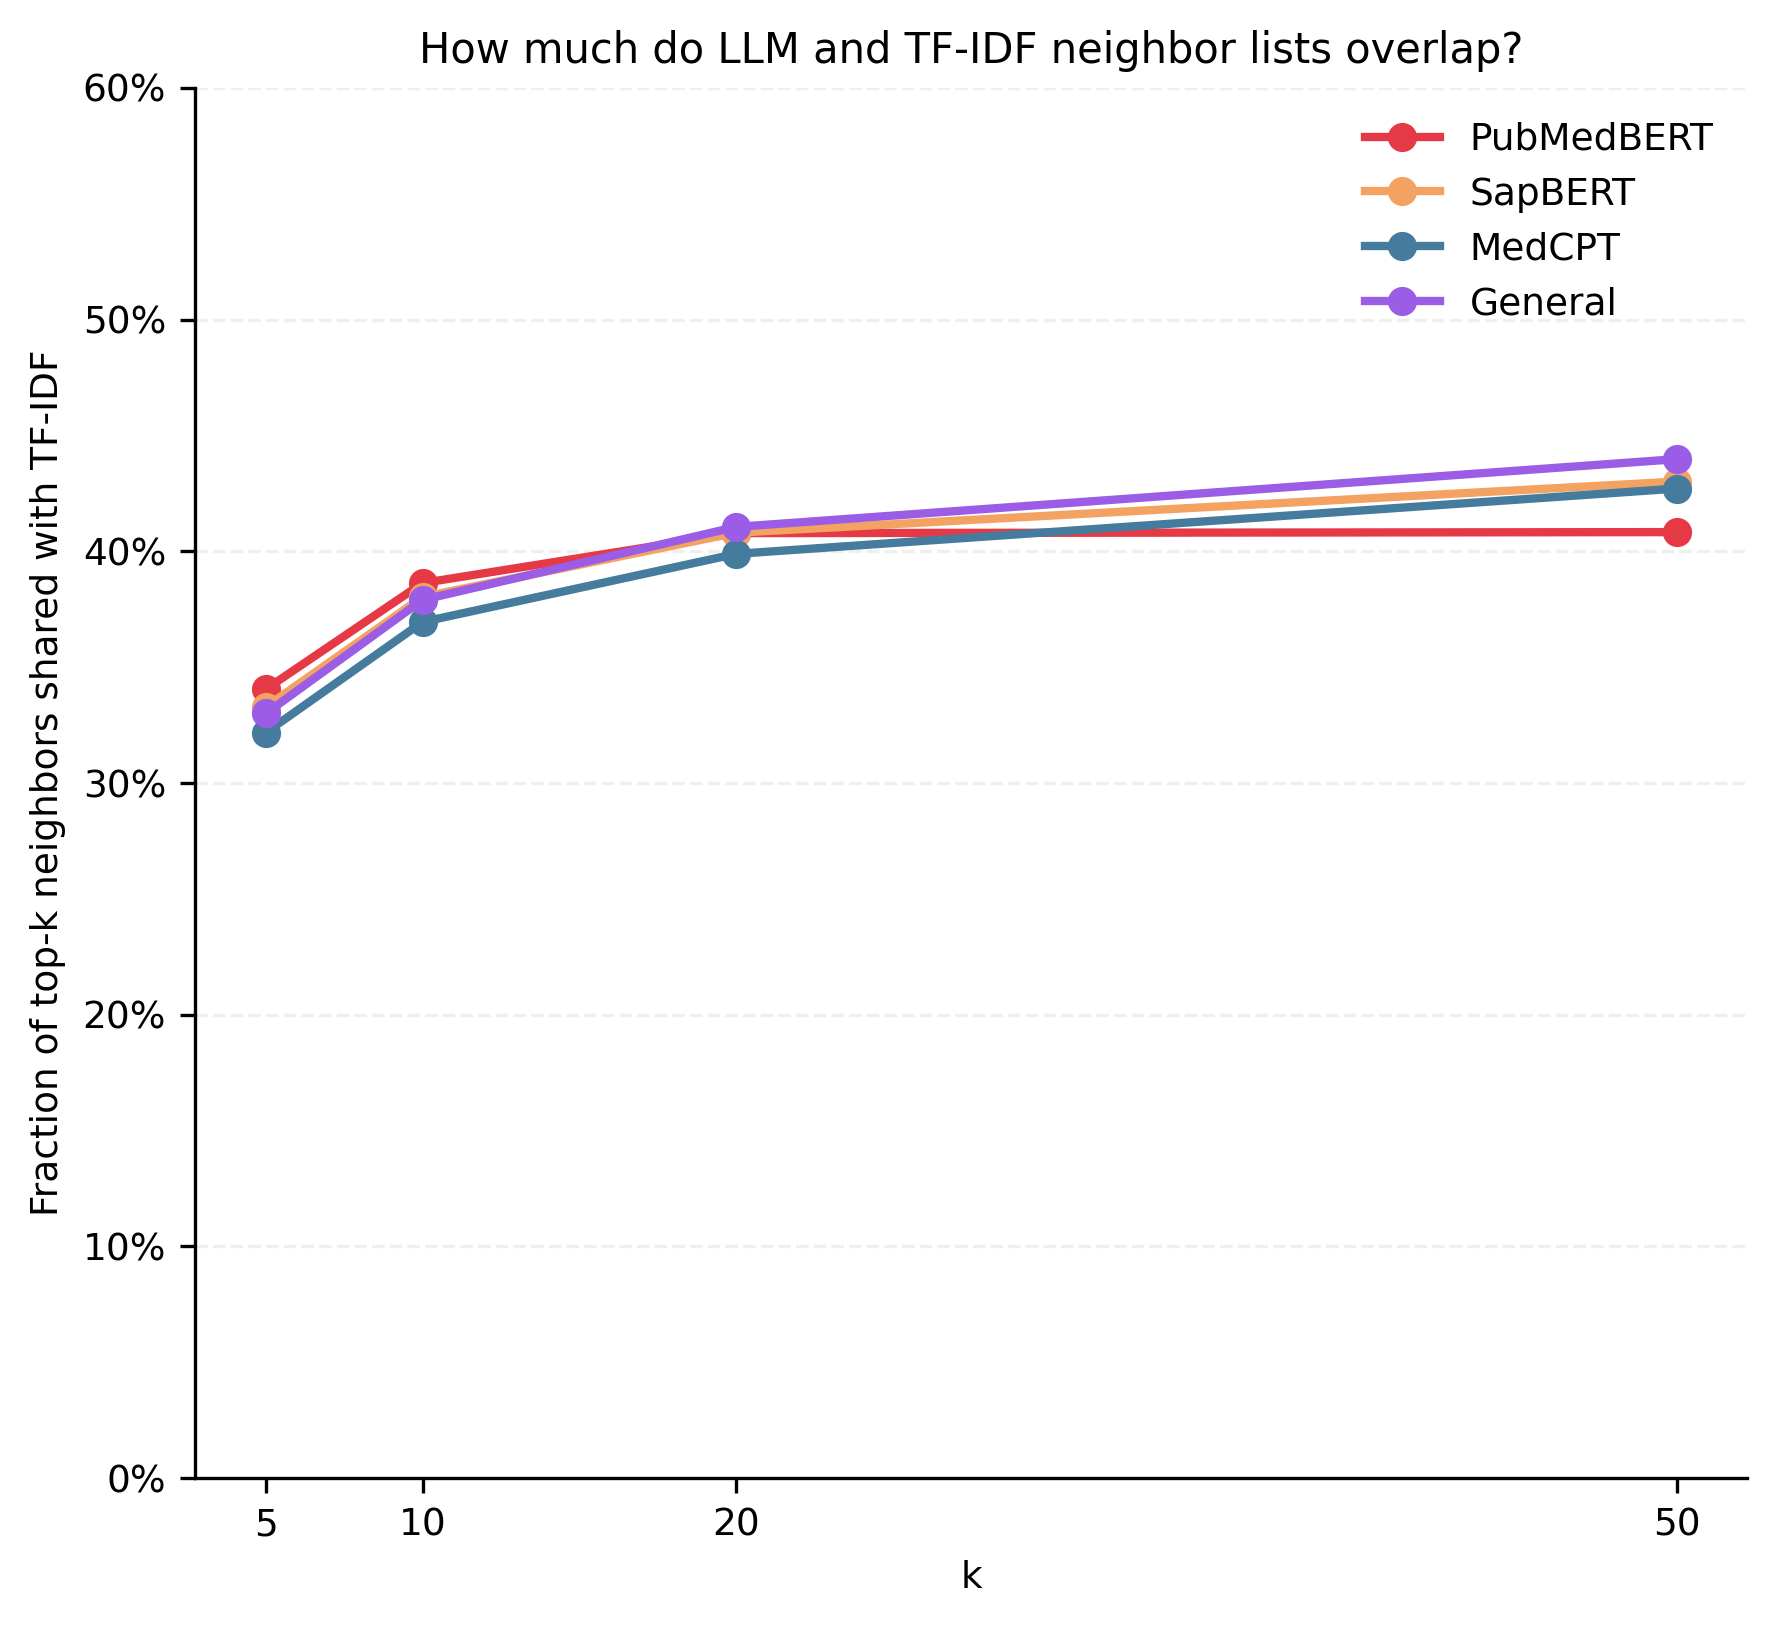
\includegraphics[width=\columnwidth]{fig4b.png}
  \caption{All 32,245 experiments (contrast analysis). Fraction of top-$k$
  LLM nearest neighbors shared with TF-IDF ($\sim$33\% at $k=5$; 44--45\% in
  well-covered experiments).}
  \label{fig:decomp_b}
\end{figure}

\begin{figure}[!t]
  \centering
  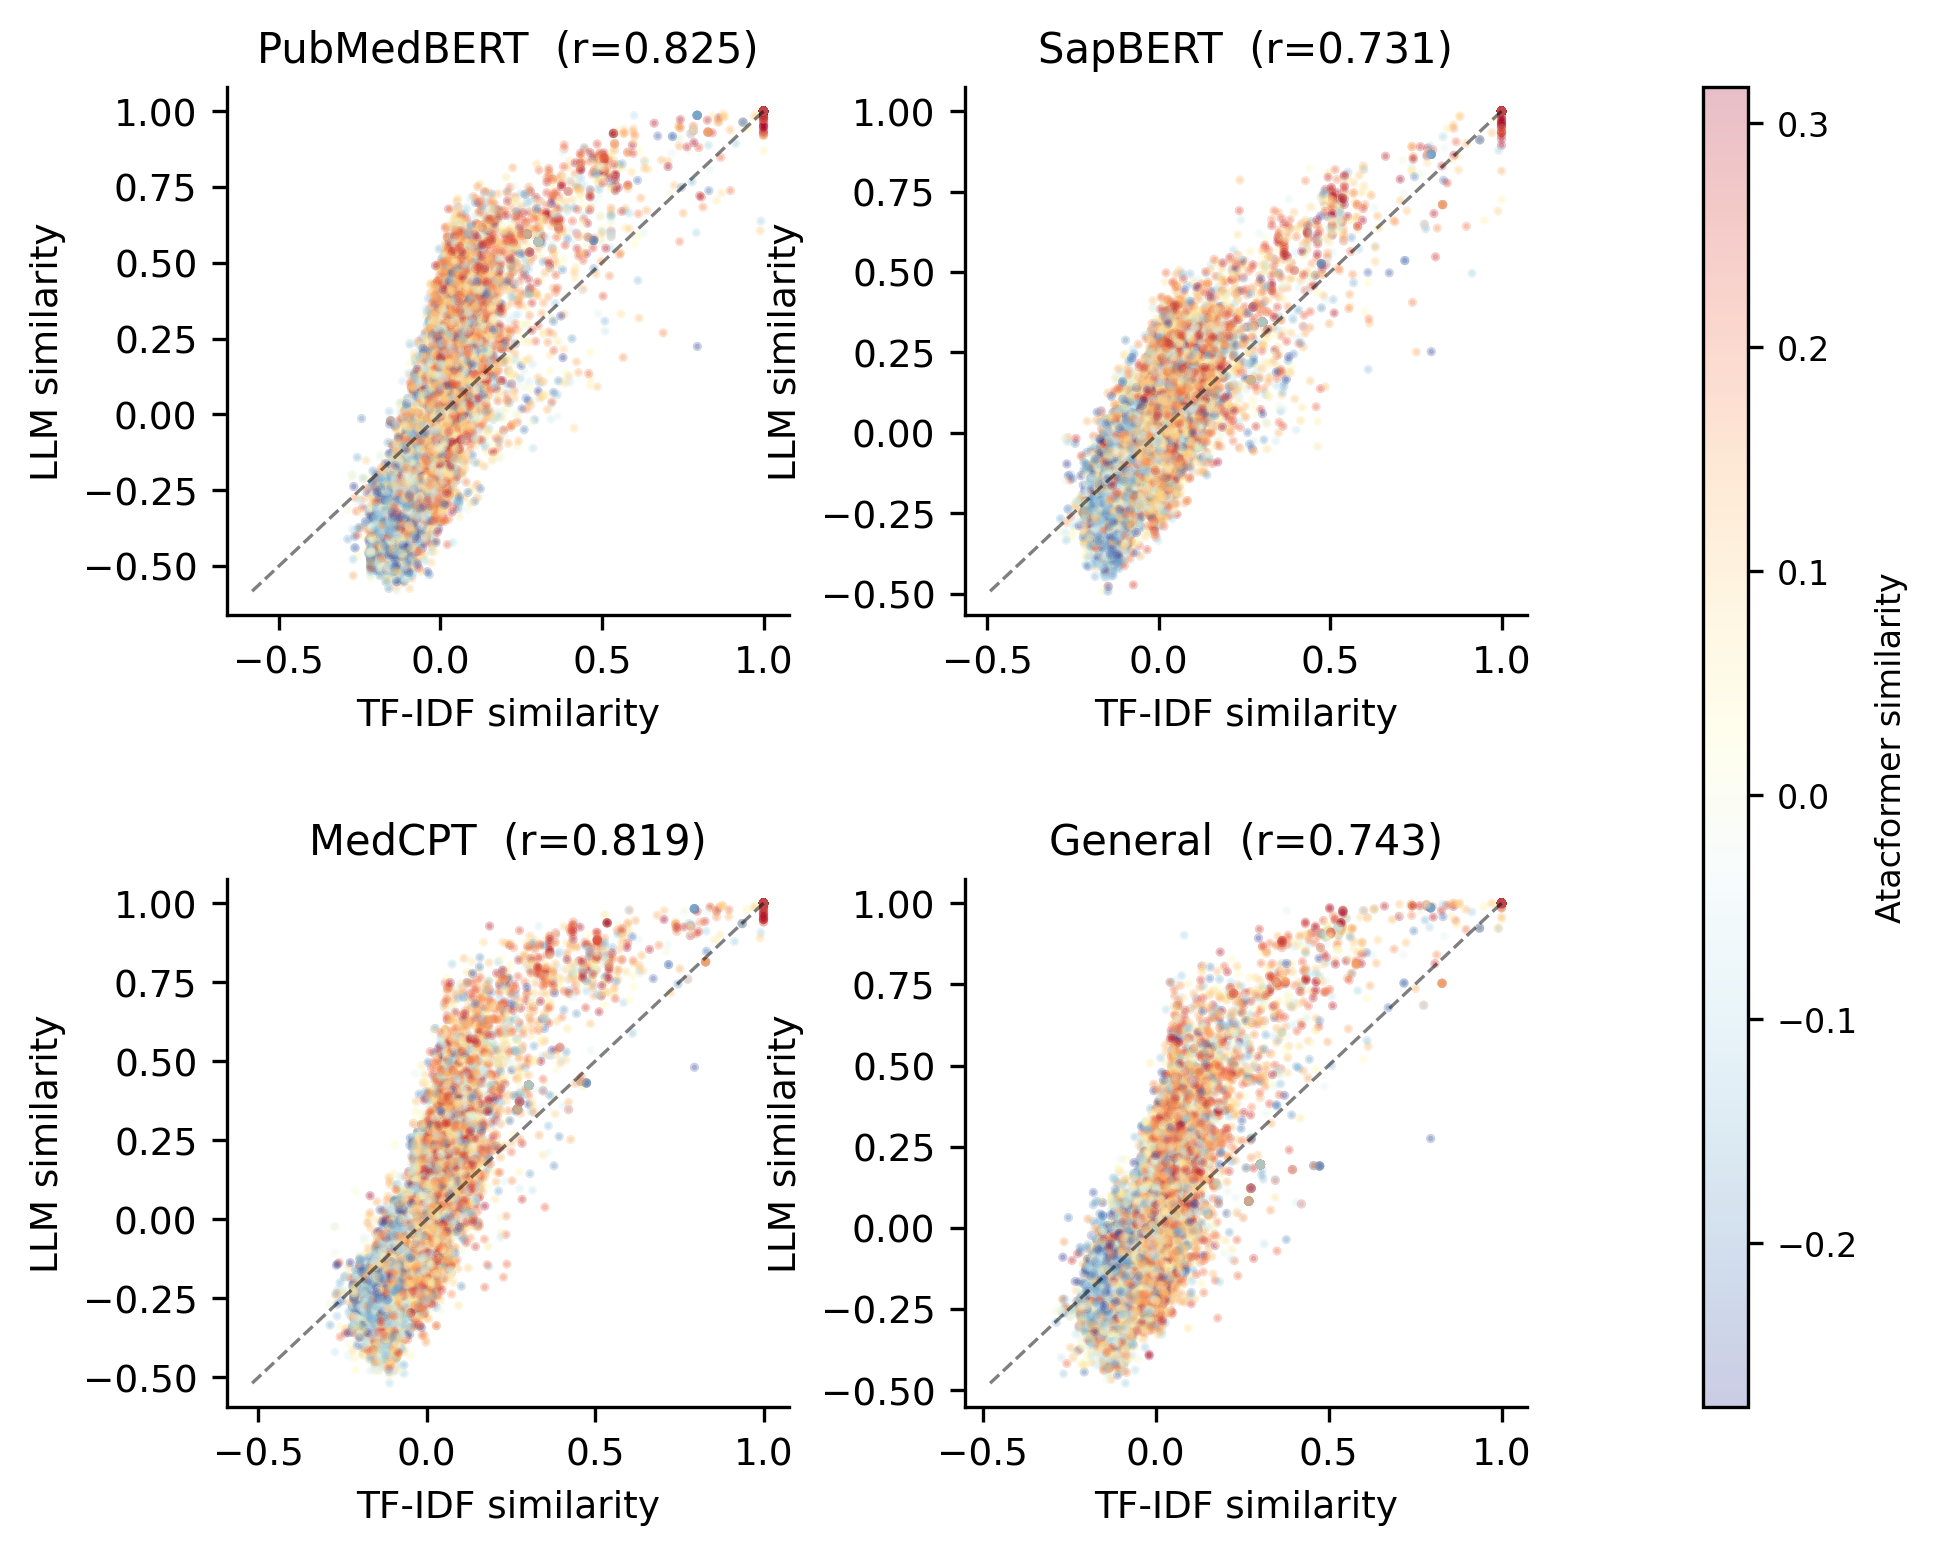
\includegraphics[width=\columnwidth]{figS3a.png}
  \caption{All 32,245 experiments (contrast analysis). TF-IDF ($x$-axis)
  vs.\ LLM ($y$-axis) pairwise similarity for 25,000 randomly sampled
  experiment pairs, colored by Atacformer similarity (RdYlBu; warmer = higher).
  Points above the diagonal indicate pairs the LLM scores higher than TF-IDF.}
  \label{fig:s3a}
\end{figure}

\begin{figure}[!t]
  \centering
  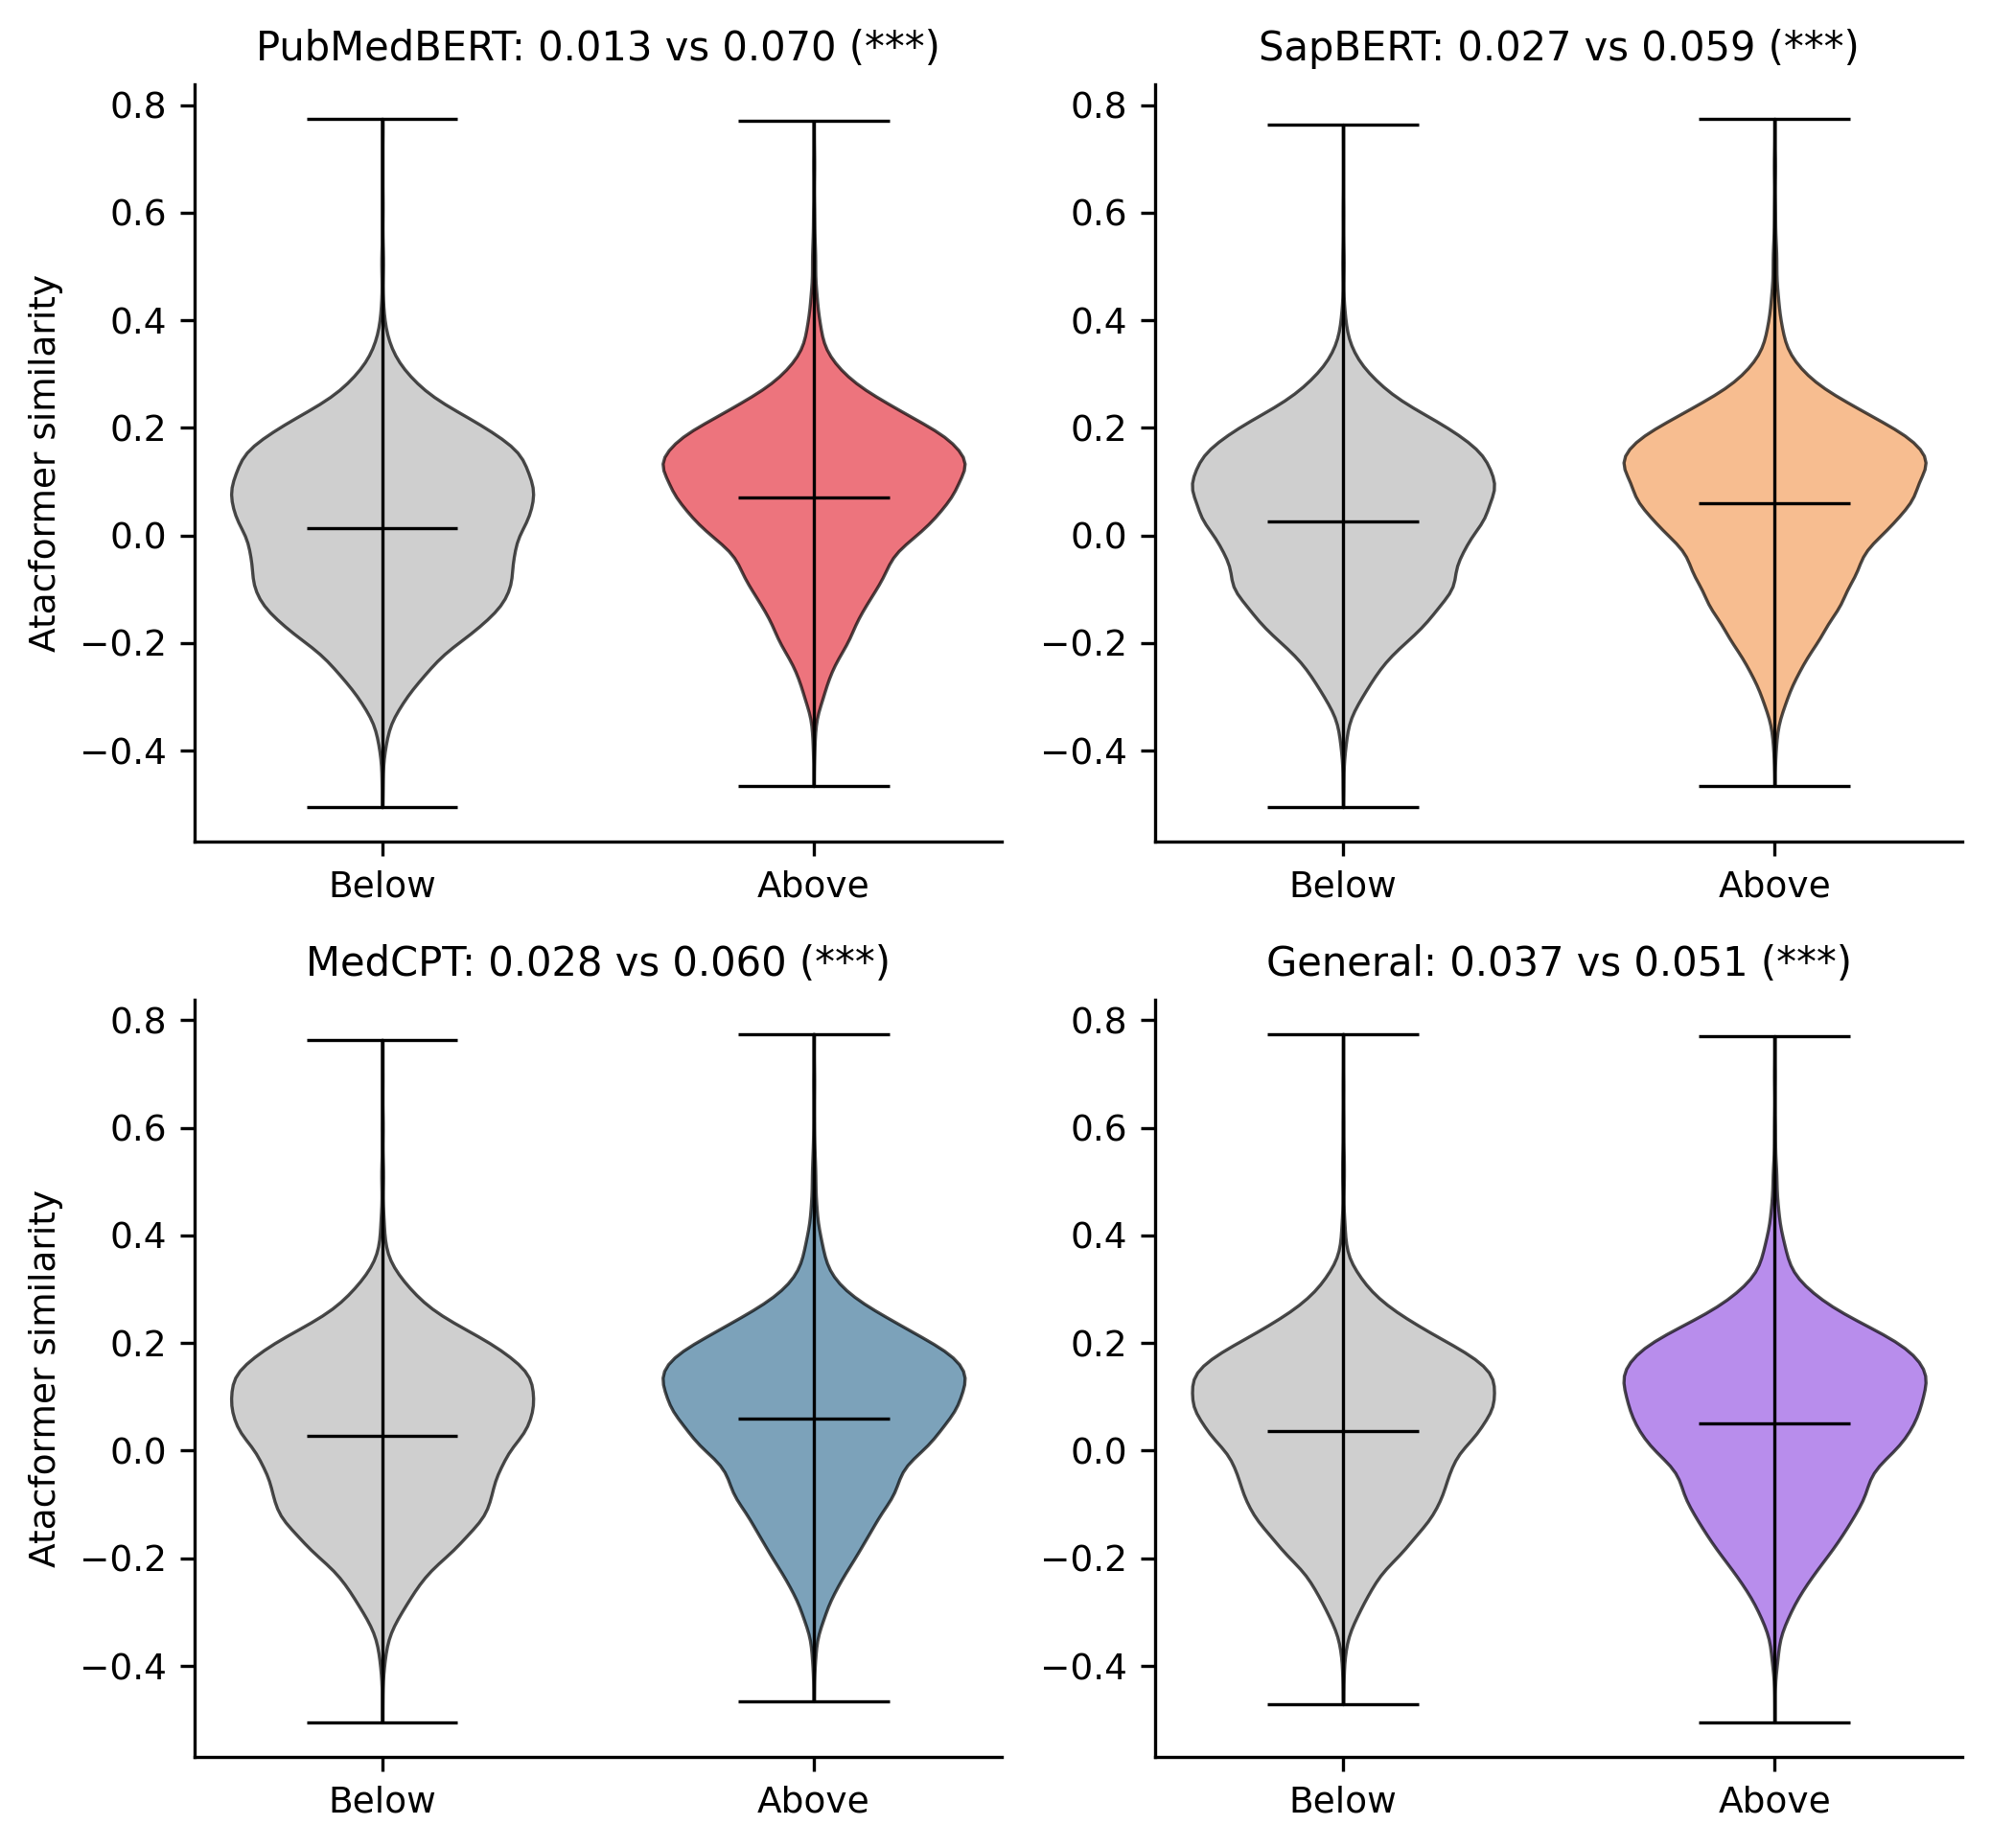
\includegraphics[width=\columnwidth]{figS3b.png}
  \caption{All 32,245 experiments (contrast analysis). Atacformer similarity
  for below- vs.\ above-diagonal pairs in Fig.~\ref{fig:s3a} (Welch's
  $t$-test). For all four models, above-diagonal pairs have higher mean
  Atacformer similarity (PubMedBERT: 0.070 vs.\ 0.013; SapBERT: 0.059 vs.\
  0.027; MedCPT: 0.060 vs.\ 0.028; General: 0.051 vs.\ 0.037); $d$ denotes
  Cohen's $d$ effect size (PubMedBERT: $d=0.38$; SapBERT: $d=0.22$; MedCPT:
  $d=0.21$; General: $d=0.09$).}
  \label{fig:s3b}
\end{figure}

\subsection{Text Shares Local Structure with RP but Not Atacformer}

Top-$k$ neighborhood overlap sharpened the contrast between the two
references. In well-covered experiments, full-text models shared 31 to 35\%
of their top-5 neighbors with RP (PubMedBERT: 34.7\%; SapBERT: 34.2\%;
General: 32.8\%; MedCPT: 30.9\%; TF-IDF: 28.2\%; name-only models: about
12\%), but less than 0.1\% with Atacformer (chance: 0.03\%). Atacformer and RP
themselves shared only 0.1\% of top-5 neighbors. On the full dataset, the
corresponding values were 20 to 23\% for RP and 2 to 3\% for Atacformer
(Figs.~\ref{fig:topk}--\ref{fig:s2}).

Neighborhood purity explains this dissociation. In well-covered experiments,
76\% of an experiment's top-5 RP neighbors shared its cell-type label
(text models: 93 to 96\%), compared with 1.3\% for Atacformer, barely above the
0.8\% expected by chance (full dataset: RP 72\%, Atacformer 21\%). Within
well-covered experiments, Atacformer similarity was no longer associated with
depth match ($r = 0.06$), whereas RP similarity still was ($r = 0.57$).
RP experiments of the same cell type were far more self-similar than
Atacformer experiments (median within-cell-type similarity 0.51 vs.\ 0.17
across 796 cell types; Atacformer lower for 96.7\%; Wilcoxon signed-rank
$p = 1.1 \times 10^{-125}$; full-dataset values in
Figs.~\ref{fig:s4}--\ref{fig:s4b}).

RP therefore encodes cell-type identity that text metadata also captures,
but it remains sensitive to peak count. The Atacformer embeddings used here,
by contrast, carry little cell-type information for peak-rich experiments, so
their low agreement with text should not be read as evidence that Atacformer
captures finer biological variation that text misses. One possible
explanation, which we did not test, is that each embedding summarizes at most
1,024 randomly sampled peaks (Section~\ref{sec:atacformer}), a small and variable fraction of
the peaks in a well-covered experiment.

\begin{figure}[!t]
  \centering
  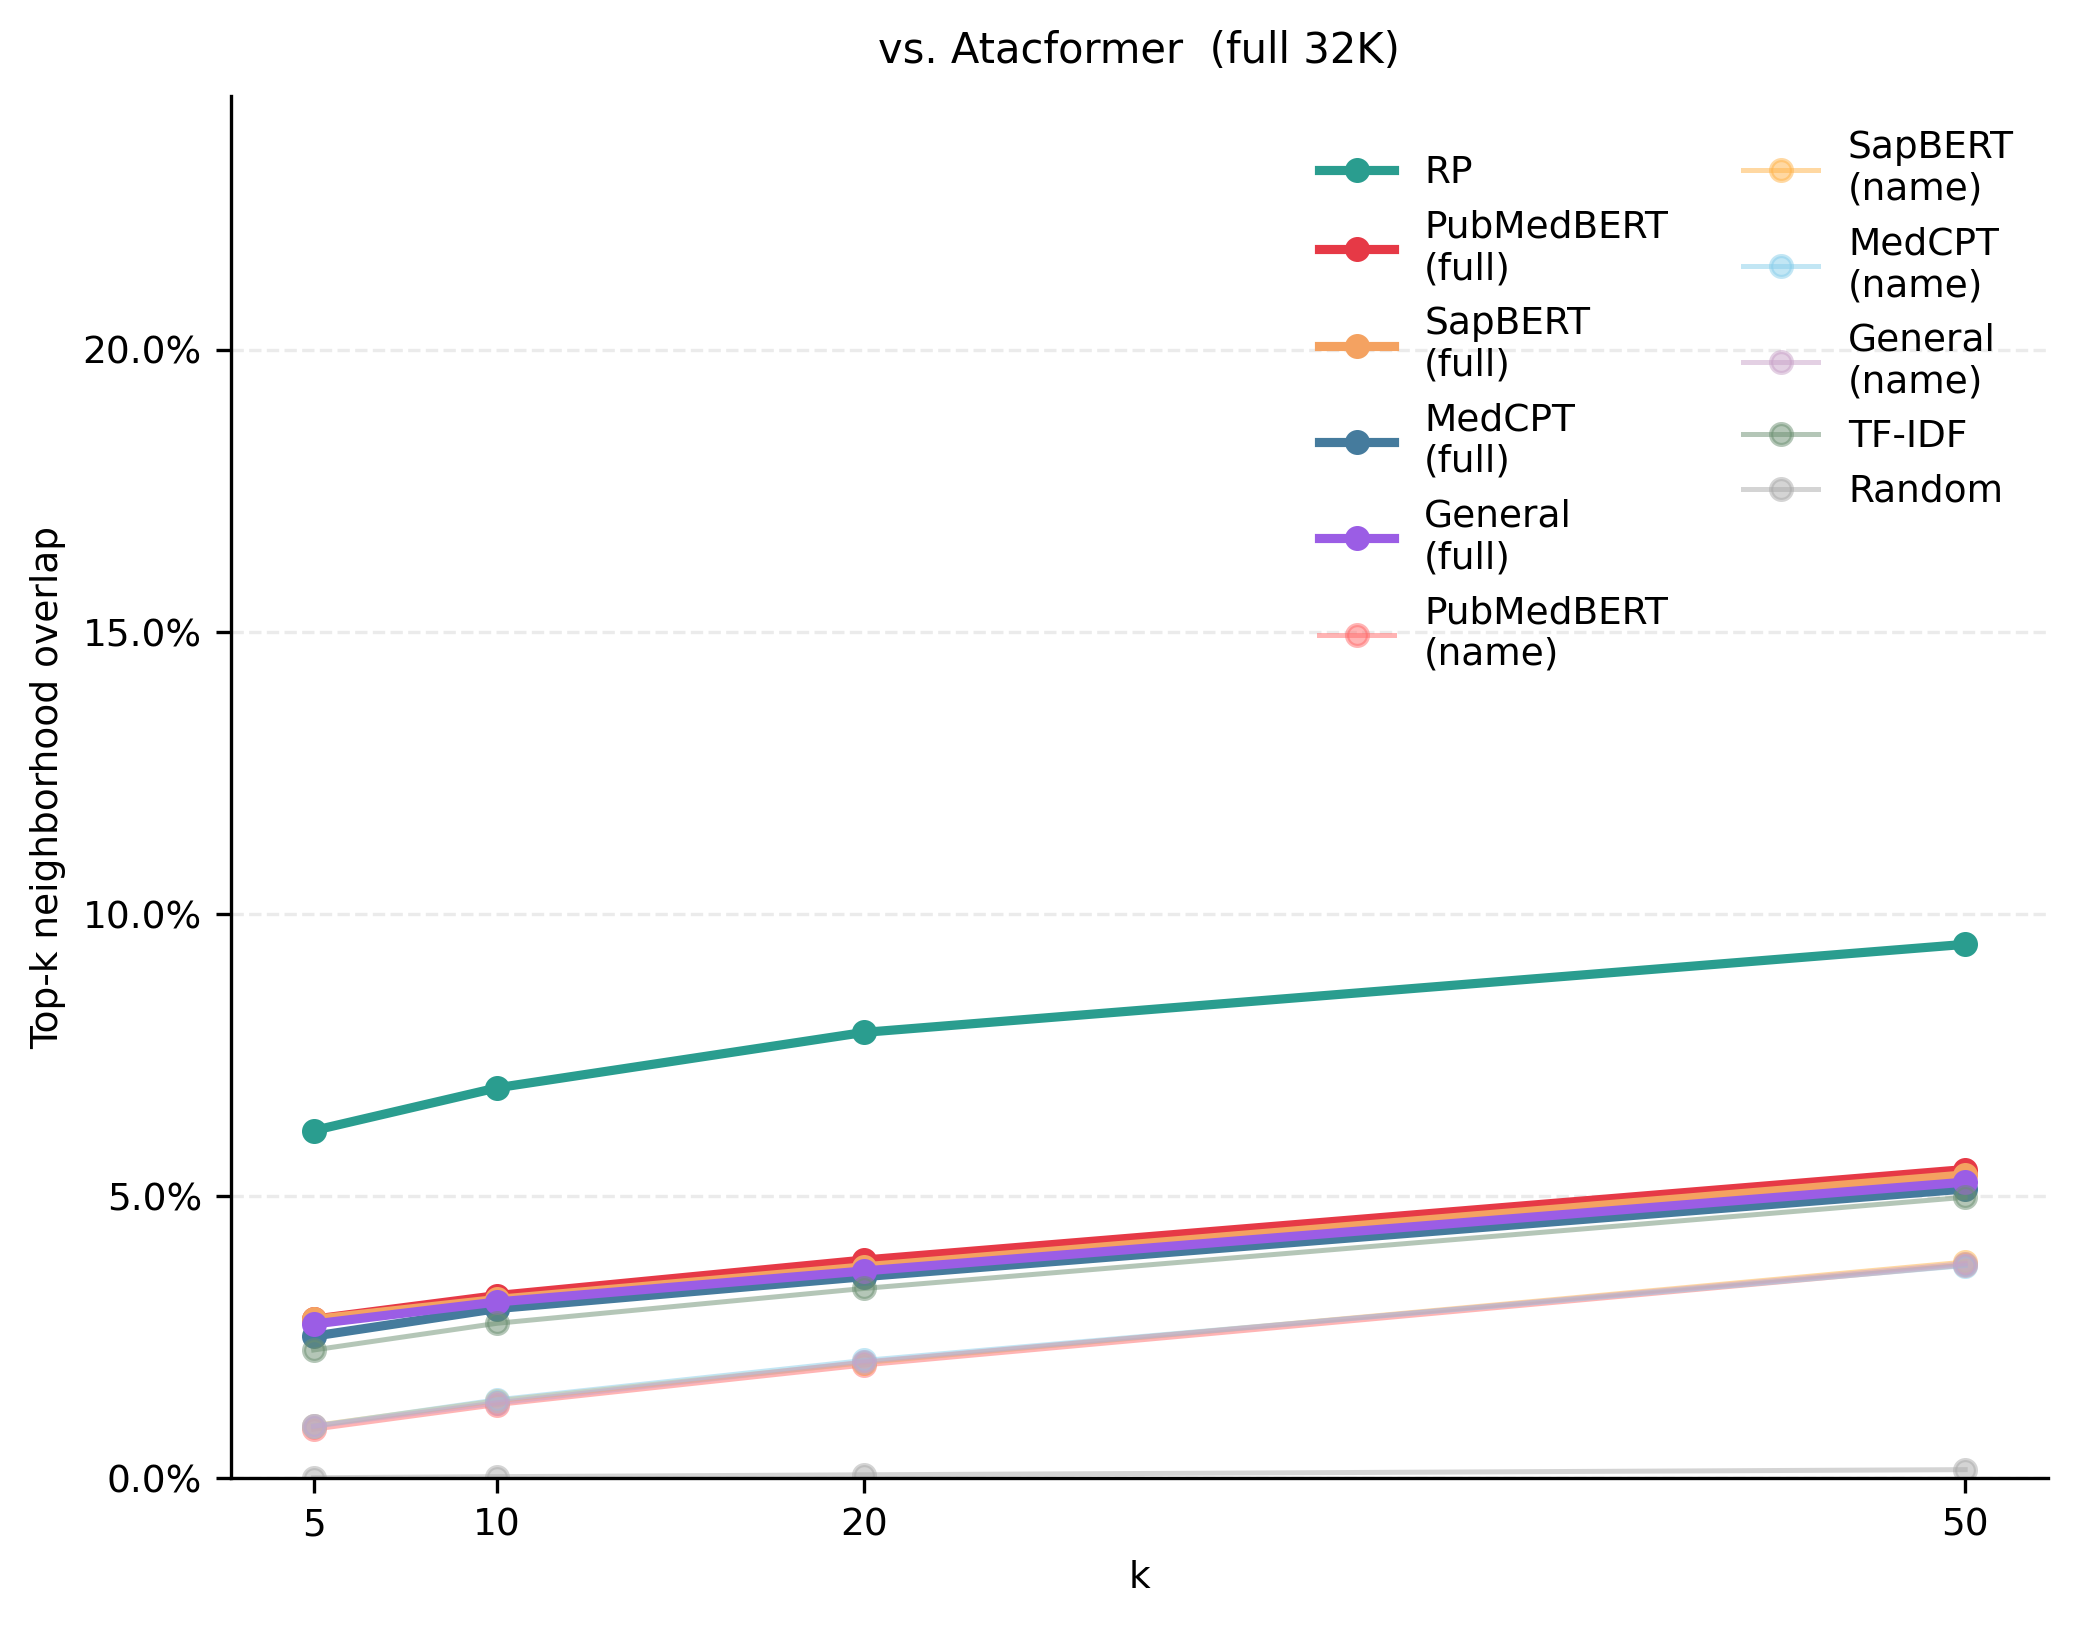
\includegraphics[width=\columnwidth]{fig3a.png}
  \caption{All 32,245 experiments (contrast analysis). Top-$k$ neighborhood
  overlap vs.\ Atacformer. Full-text models share $\sim$2 to 3\% of nearest
  neighbors with Atacformer at $k=5$ ($<$0.1\% in well-covered experiments).}
  \label{fig:topk}
\end{figure}

\begin{figure}[!t]
  \centering
  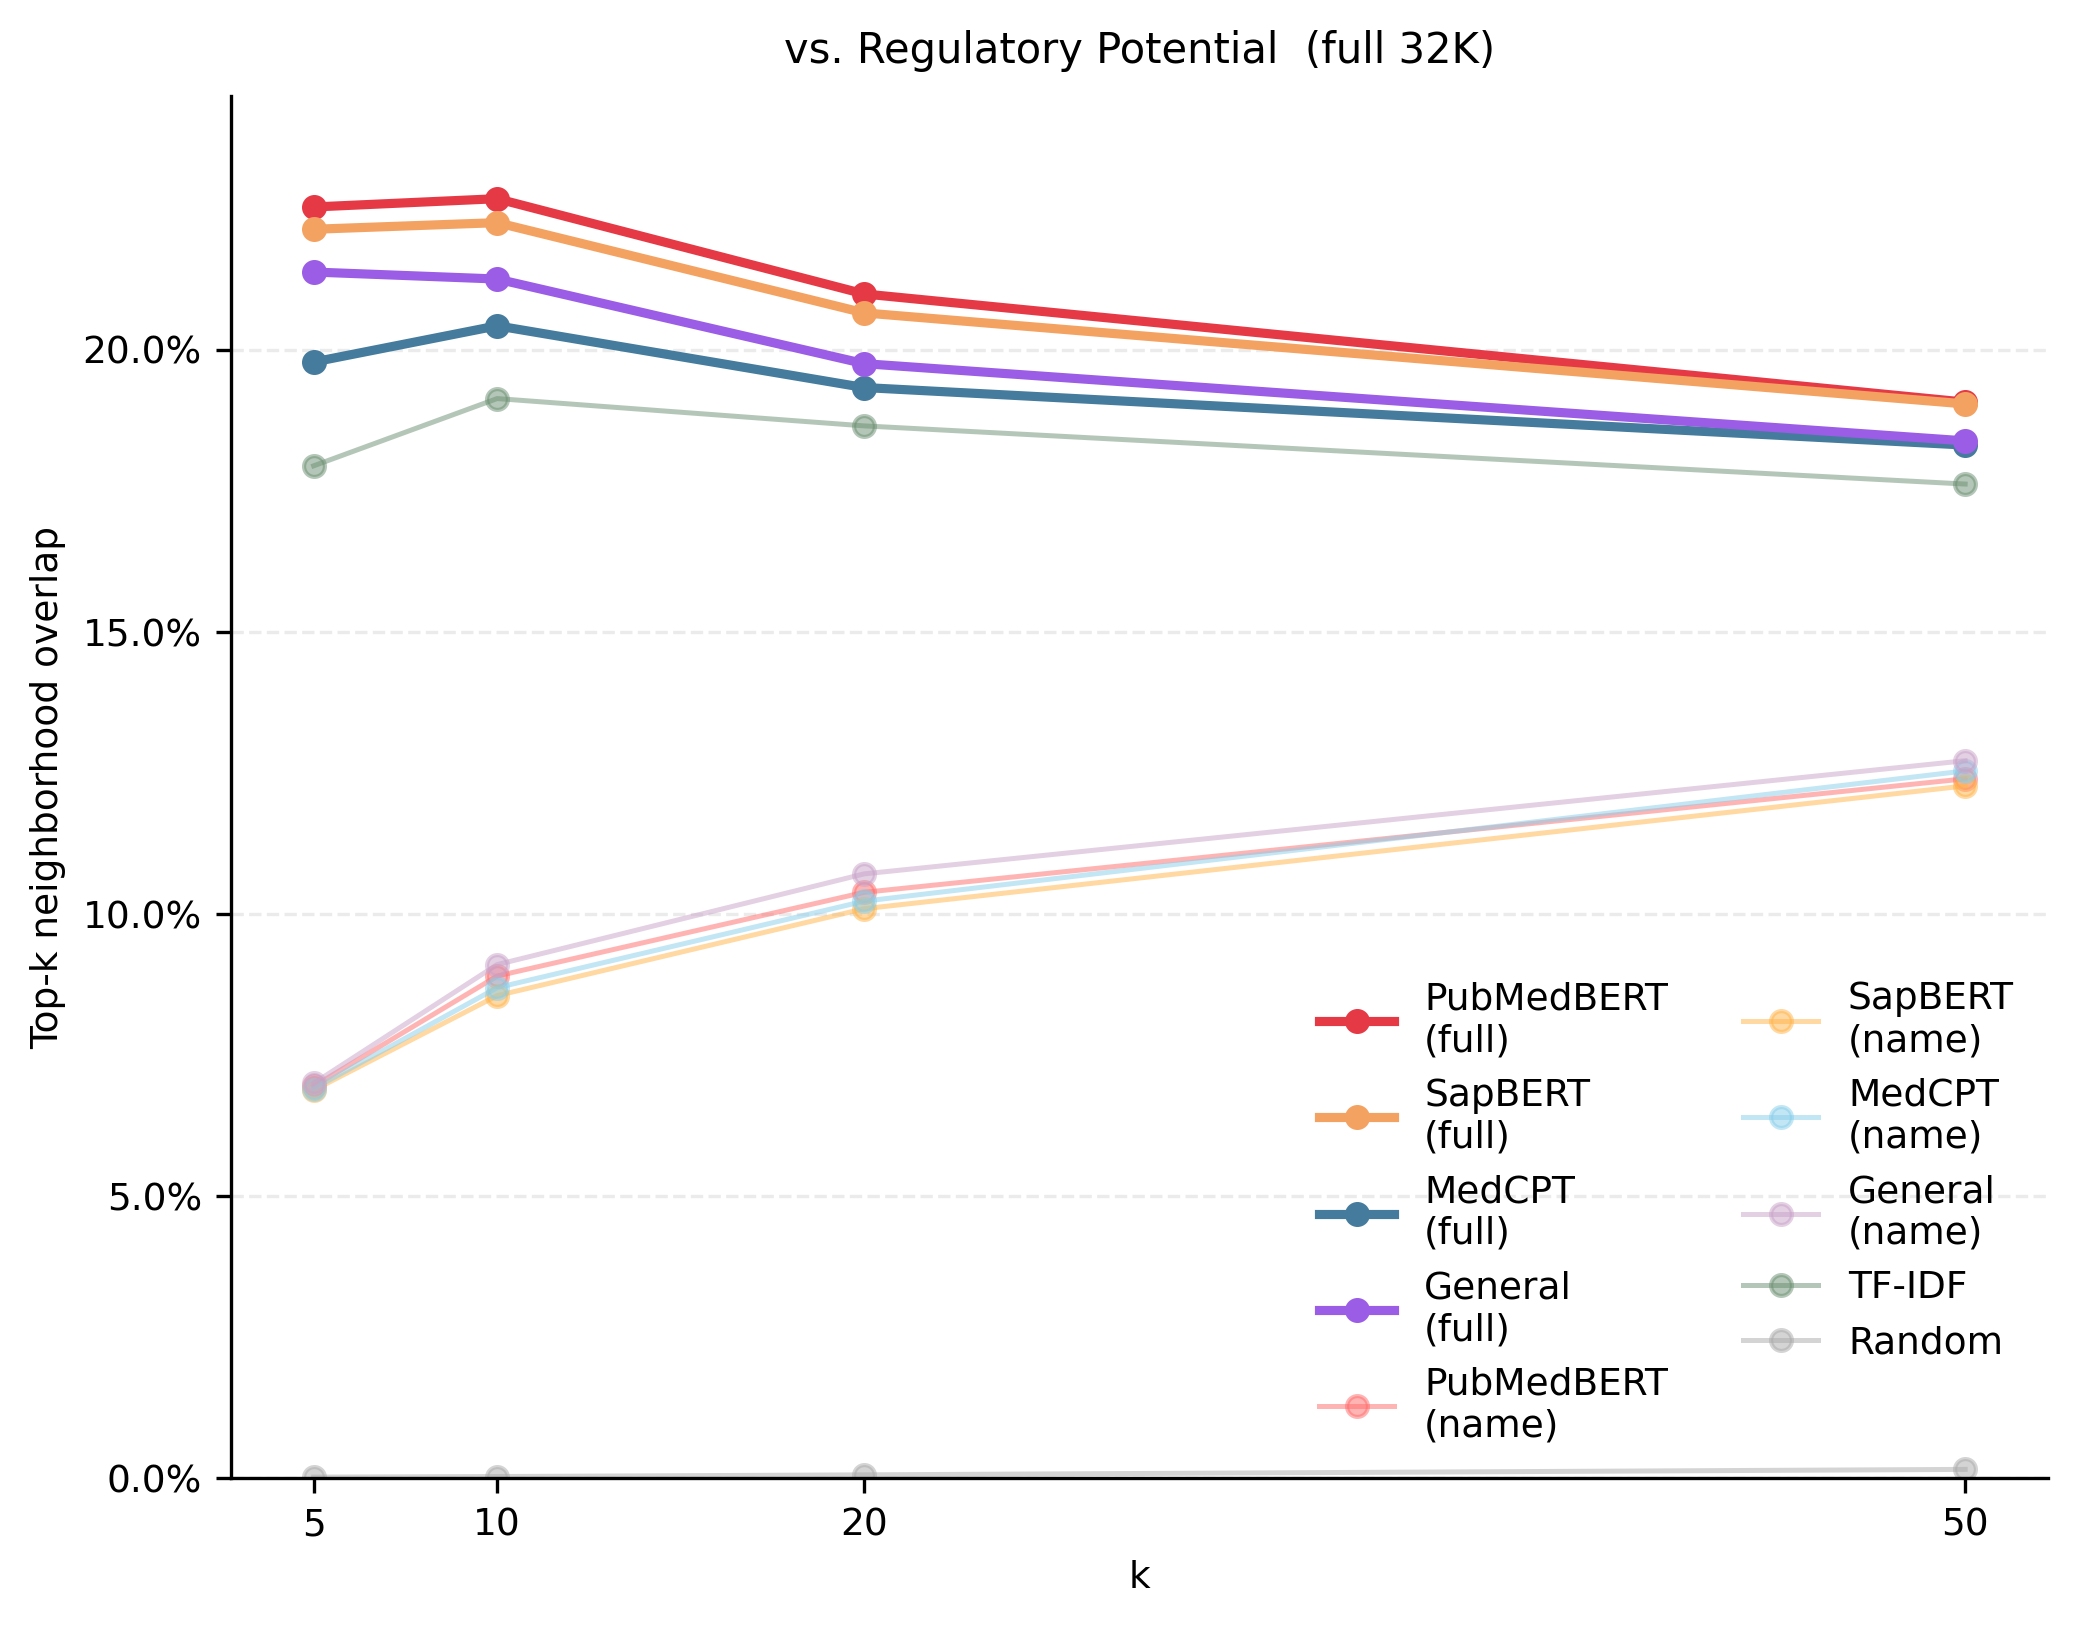
\includegraphics[width=\columnwidth]{fig3b.png}
  \caption{All 32,245 experiments (contrast analysis). Top-$k$ neighborhood
  overlap vs.\ regulatory potential (RP). Full-text models share $\sim$20 to
  23\% of nearest neighbors with RP at $k=5$ (31 to 35\% in well-covered
  experiments).}
  \label{fig:topk_rp}
\end{figure}

\begin{figure}[!t]
  \centering
  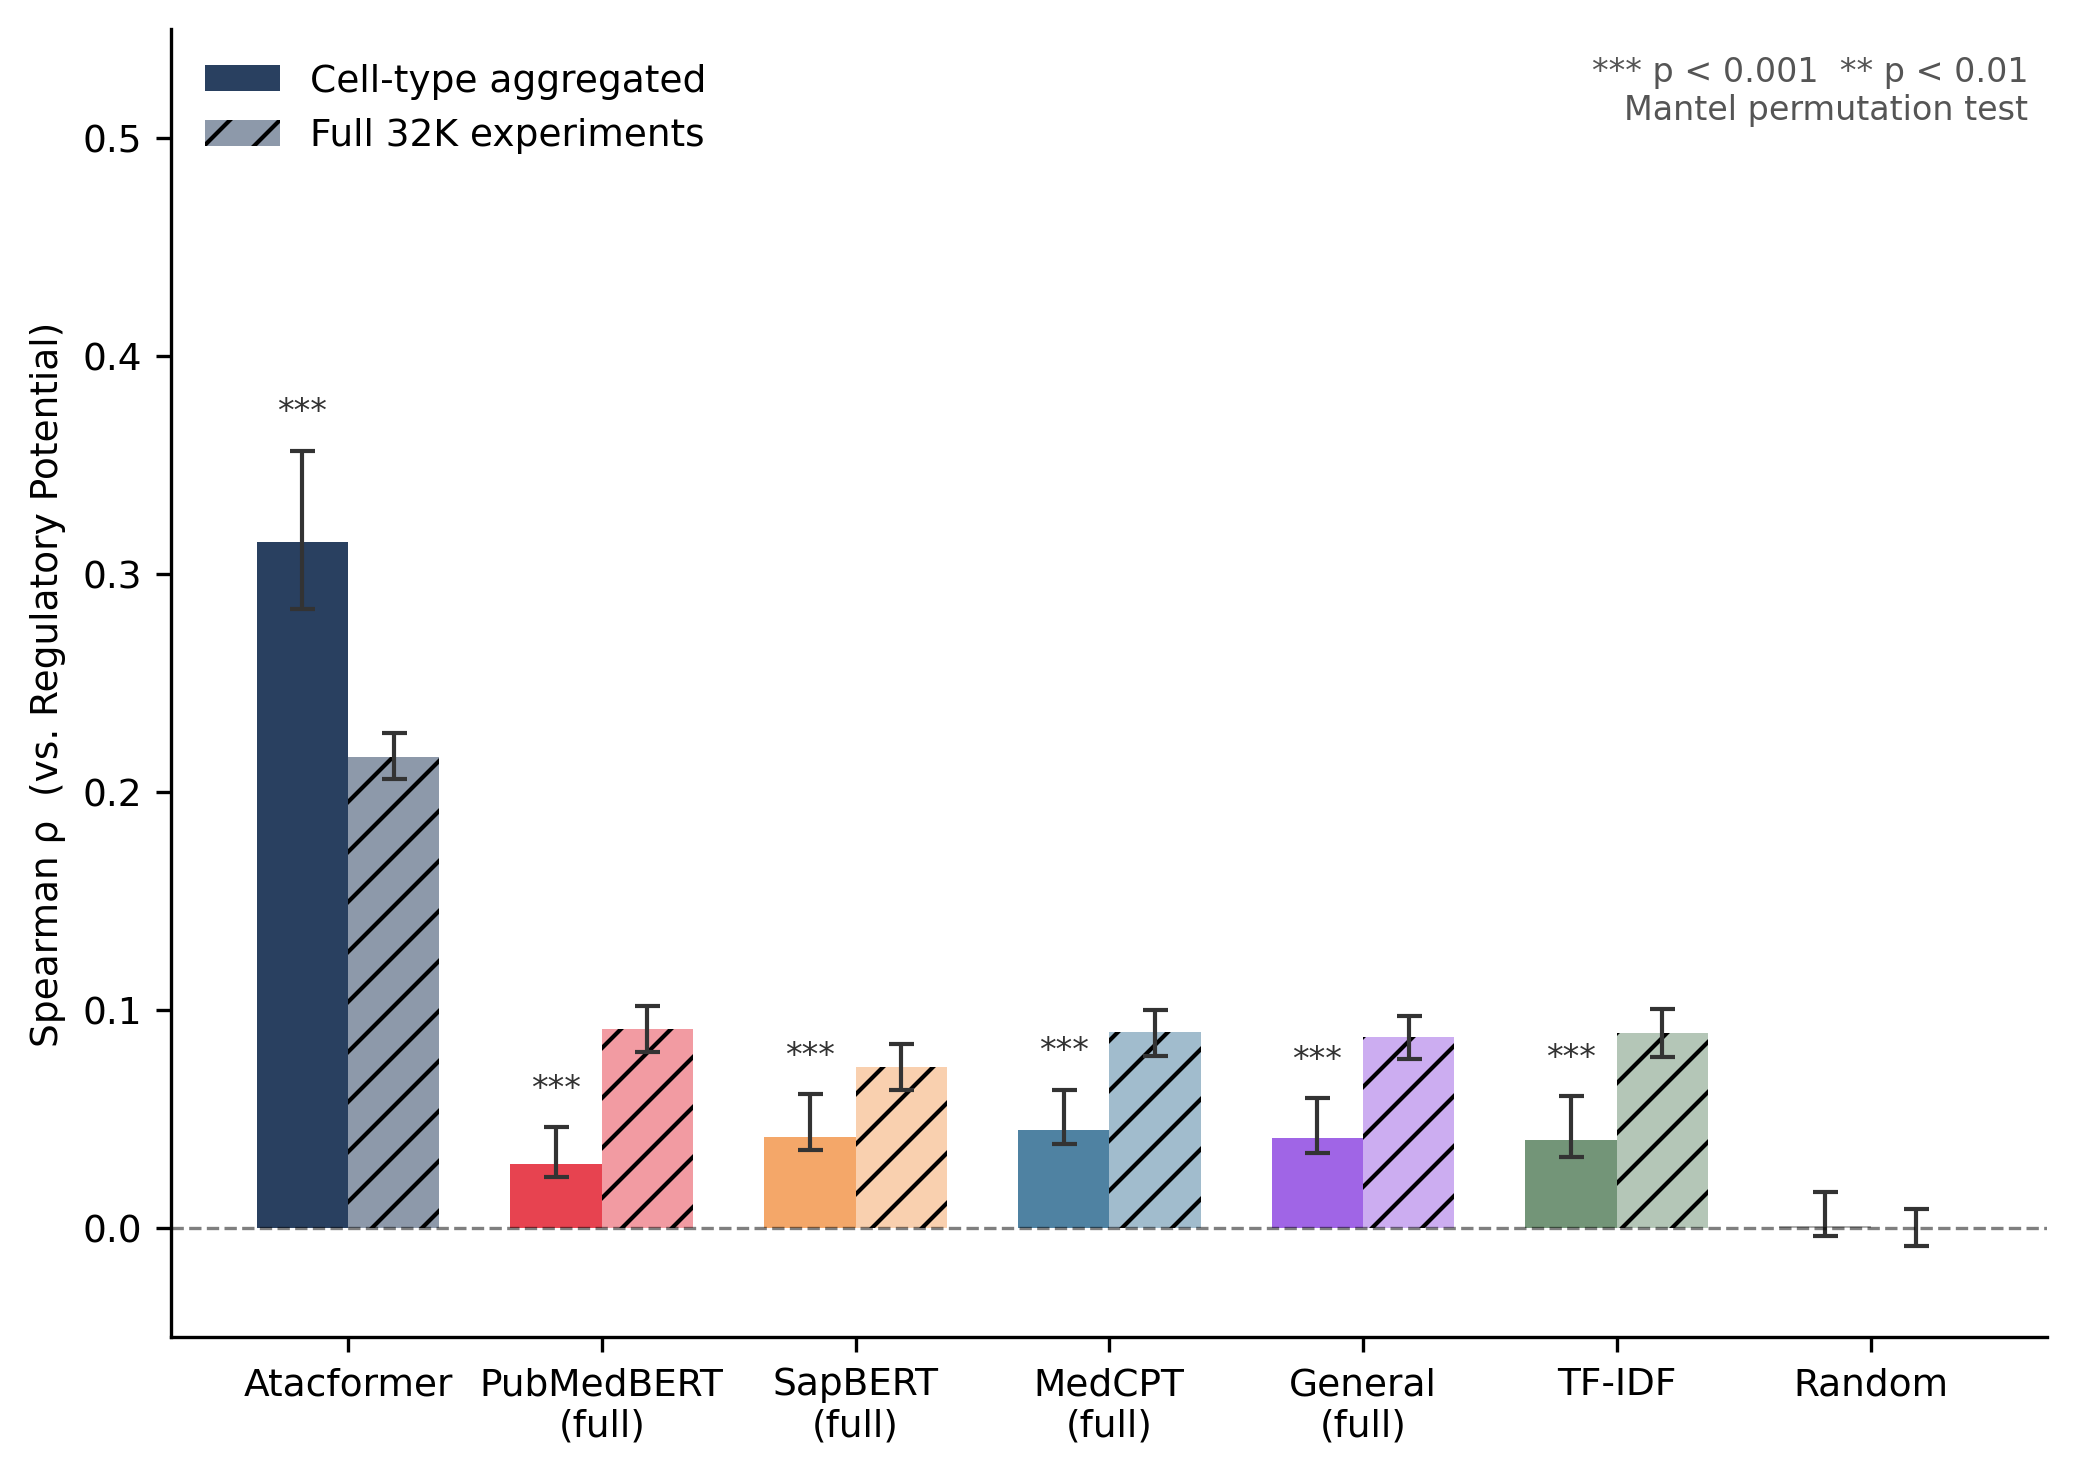
\includegraphics[width=\columnwidth]{figS2n.png}
  \caption{All 32,245 experiments (contrast analysis). Spearman rank
  correlation between each embedding type and regulatory potential (RP)
  (name-only variants omitted for clarity). Error bars show 95\% bootstrap
  confidence intervals; significance markers (Mantel permutation test) are
  shown for the cell-type-aggregated bars only. Well-covered results are in
  Table~\ref{tab:spearman}.}
  \label{fig:s2}
\end{figure}

\begin{figure}[!t]
  \centering
  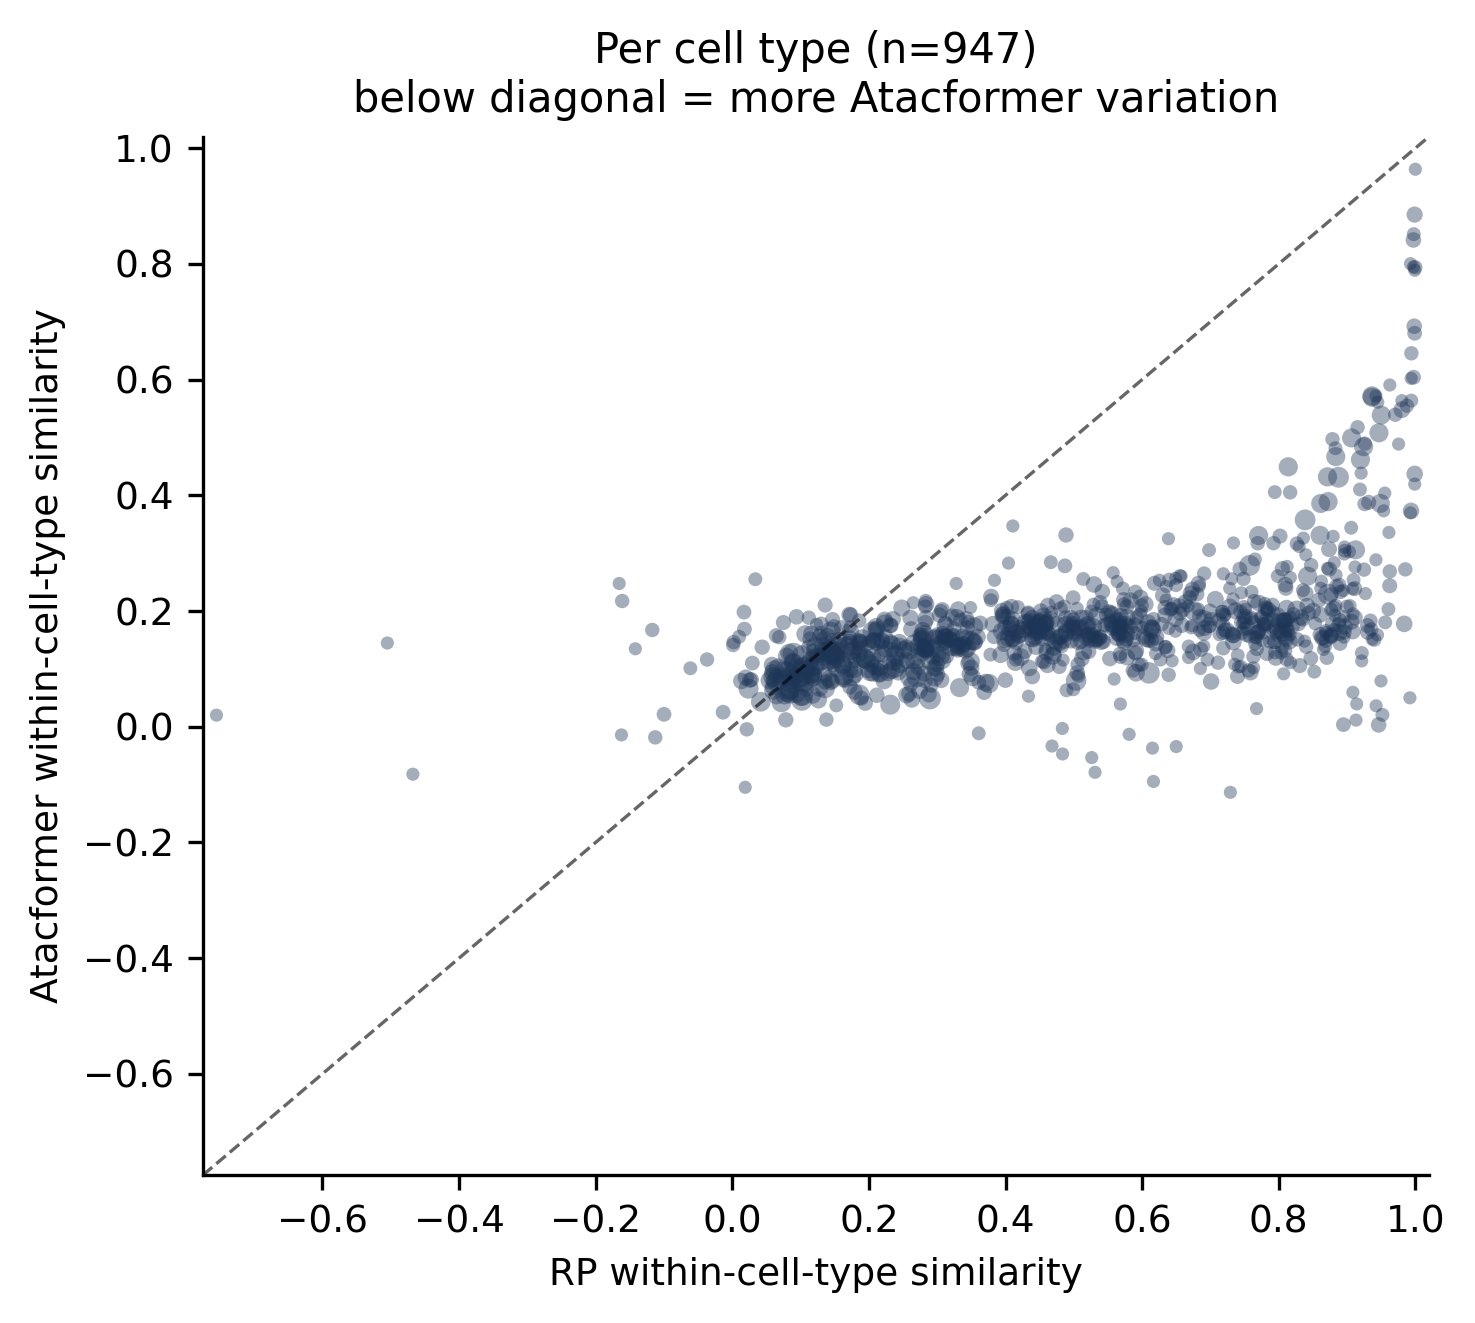
\includegraphics[width=\columnwidth]{figS4a.png}
  \caption{All 32,245 experiments (contrast analysis). Per-cell-type
  within-cell-type similarity for Atacformer vs.\ RP, computed as mean pairwise
  cosine similarity among experiments sharing a cell-type label (947 cell types
  with $\geq 2$ experiments). Points below the diagonal indicate lower
  within-cell-type similarity for Atacformer than RP.}
  \label{fig:s4}
\end{figure}

\begin{figure}[!t]
  \centering
  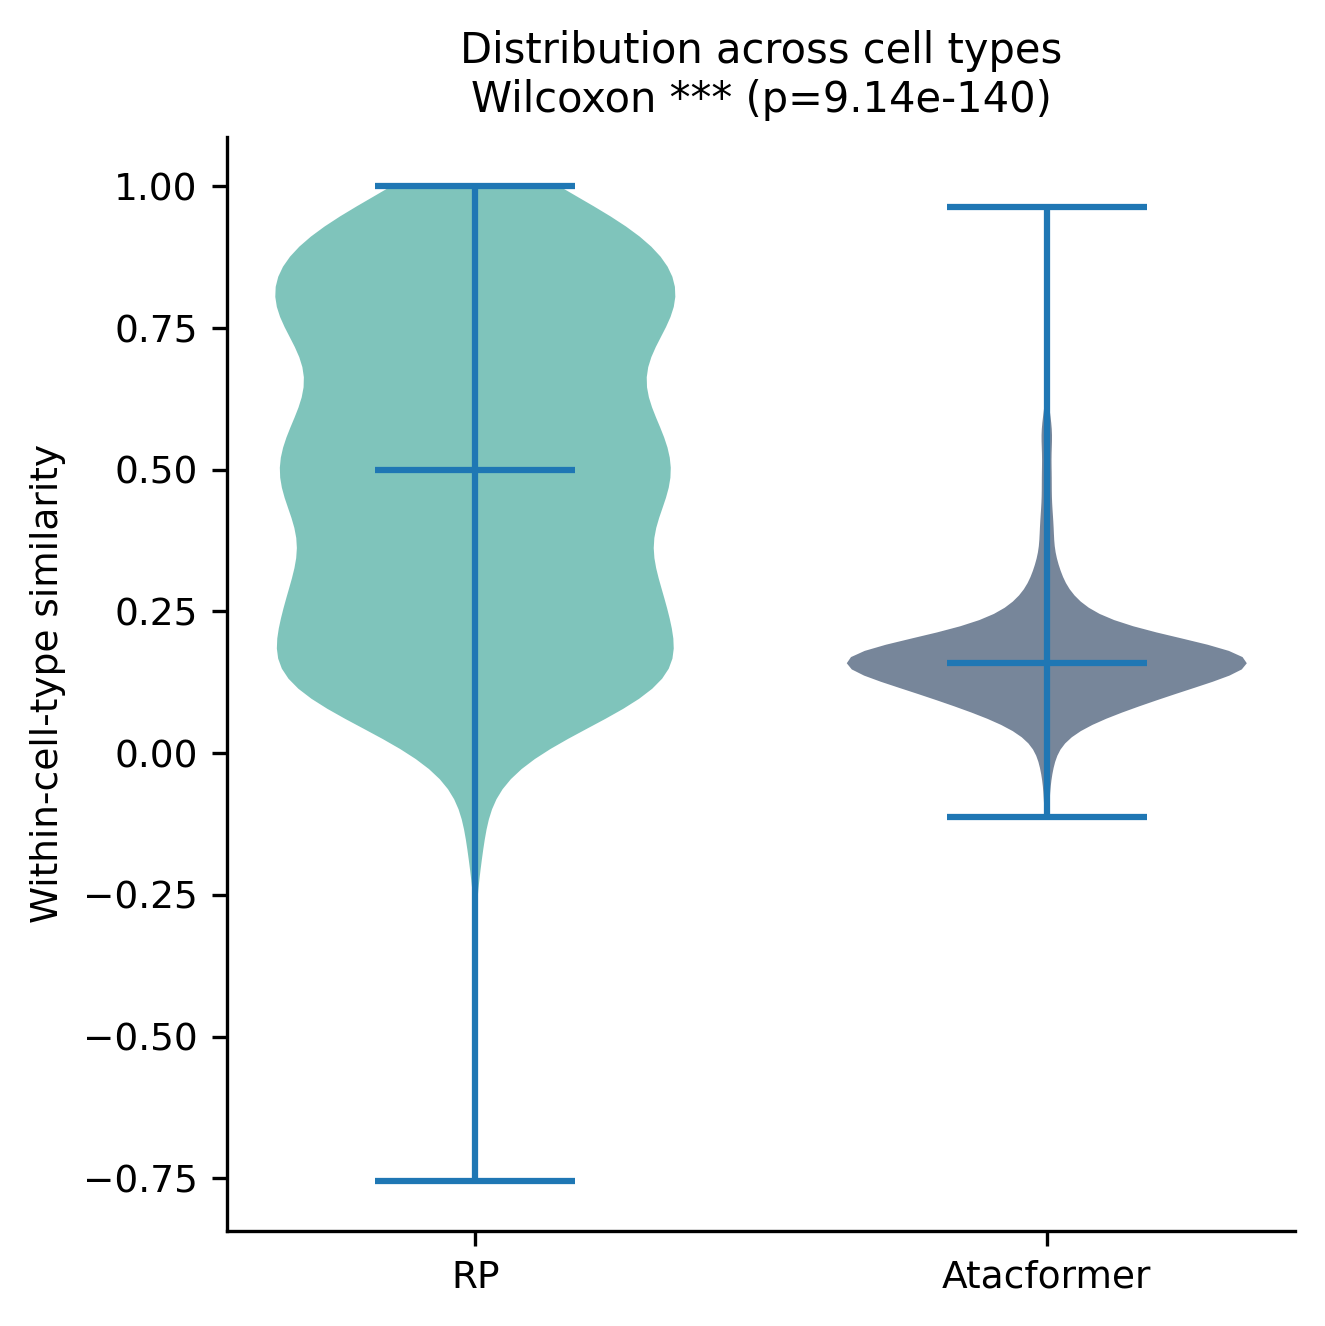
\includegraphics[width=\columnwidth]{figS4b.png}
  \caption{All 32,245 experiments (contrast analysis). Distribution of
  within-cell-type similarity across cell types (Wilcoxon signed-rank test;
  RP median 0.50, Atacformer median 0.16). Within-cell-type similarity tracks
  the spread of peak counts within each cell type
  (Section~\ref{sec:coverage}).}
  \label{fig:s4b}
\end{figure}

\FloatBarrier
\begin{table*}[!t]
  \centering\footnotesize
  \setlength{\tabcolsep}{4pt}
  \begin{minipage}[t]{0.48\linewidth}
    \centering
    \caption{All 32,245 experiments (contrast analysis). Experiment pairs with
    high Atacformer similarity (top 5\%) and low TF-IDF similarity (below
    median). The leading pair (NCI-H1299 / CD4+ T cells) consists of two
    low-peak experiments (1,181 and 1,272 peaks; corpus median 6,287).
    ``(unlabeled)'' denotes experiments lacking a cell-type annotation in
    ChIP-Atlas.}
    \label{tab:qual_atac}
    \begin{tabular}{llcc}
      \toprule
      Cell type A & Cell type B & Atac. & TFIDF \\
      \midrule
      NCI-H1299            & CD4+ T cells              & $0.374$ & $-0.196$ \\
      iPSC derived cells   & PC-9                      & $0.361$ & $-0.176$ \\
      NCI-H1648            & iMeLCs                    & $0.312$ & $-0.214$ \\
      (unlabeled)          & CD4+ T cells              & $0.398$ & $-0.147$ \\
      NCI-H1648            & iPSC neural cells         & $0.307$ & $-0.204$ \\
      (unlabeled)          & IMR-90                    & $0.309$ & $-0.188$ \\
      (unlabeled)          & MV-4-11                   & $0.331$ & $-0.156$ \\
      (unlabeled)          & Neural crest cells        & $0.310$ & $-0.179$ \\
      iPSC derived cells   & Jurkat                    & $0.318$ & $-0.164$ \\
      (unlabeled)          & DND-41                    & $0.316$ & $-0.161$ \\
      \bottomrule
    \end{tabular}
  \end{minipage}
  \hfill
  \begin{minipage}[t]{0.48\linewidth}
    \centering
    \caption{All 32,245 experiments (contrast analysis). Experiment pairs with
    high RP similarity and low TF-IDF similarity, selected analogously to
    Table~\ref{tab:qual_atac}. Every experiment in this table has
    $\leq$1,438 peaks, i.e., these pairs reflect shared promoter signal in
    low-peak experiments rather than shared biology.}
    \label{tab:qual_rp}
    \begin{tabular}{llcc}
      \toprule
      Cell type A & Cell type B & RP & TFIDF \\
      \midrule
      iPSC derived cells & K-562           & $0.885$ & $-0.221$ \\
      NCI-H2347          & PBMC            & $0.884$ & $-0.181$ \\
      RERF-LC-Ad1        & XG-6            & $0.851$ & $-0.224$ \\
      (unlabeled)        & PKC19           & $0.901$ & $-0.171$ \\
      iPSC derived cells & T-47D           & $0.874$ & $-0.185$ \\
      (unlabeled)        & B-cell leukemia & $0.891$ & $-0.170$ \\
      NCI-H1648          & B cells         & $0.859$ & $-0.181$ \\
      NCI-H1703          & CD4+ T cells    & $0.851$ & $-0.186$ \\
      NCI-H1299          & CD4+ T cells    & $0.833$ & $-0.196$ \\
      (unlabeled)        & ES cells        & $0.916$ & $-0.154$ \\
      \bottomrule
    \end{tabular}
  \end{minipage}
\end{table*}

% ── Discussion ────────────────────────────────────────────────────────────────
\section{Discussion}

Our results establish quantitative bounds on the utility of experimental
metadata as a proxy for ATAC-seq chromatin similarity, and show that these
bounds depend critically on data quality. On the full ChIP-Atlas corpus,
text embeddings appear to correlate moderately with Atacformer similarity
($r = 0.20$ to $0.30$). This agreement is driven by low-peak experiments,
whose promoter-dominated peak sets make them resemble one another in both
chromatin representations, and by sample titles, which encode data provenance
that covaries with library quality. Among well-covered experiments, text
embeddings do not track Atacformer similarity at all.

What survives is a weak but consistent agreement between text and RP
($r = 0.06$ to $0.10$ across experiments; 31 to 35\% shared top-5
neighbors). RP neighborhoods are strongly organized by cell type, and text
metadata recovers this coarse cell-type structure. Text metadata may therefore
support coarse, cell-type-level retrieval, but it should not substitute for
chromatin similarity in fine-grained applications.

Language models add little to this signal. In well-covered experiments, TF-IDF
matches every LLM, and residual associations beyond TF-IDF are near zero for
Atacformer and small for RP. The apparent advantage of PubMedBERT and SapBERT
over MedCPT and the general encoder on the full dataset does not survive
restriction to well-covered experiments and depends on corpus centering.

These findings have a methodological implication beyond text. Peak count was
the strongest single determinant of similarity in both chromatin
representations, and it alone accounted for the agreement between Atacformer
and RP on the full dataset. Comparisons of chromatin embeddings across
heterogeneous public repositories should therefore stratify by, or control
for, peak count and related quality measures.

A central limitation is that Atacformer and RP are treated as proxies for
chromatin biology without independent validation against external ground
truth. Both are transforms of the same ChIP-Atlas peak calls, both are
sensitive to peak count, and the Atacformer embeddings used here carry little
cell-type information for well-covered experiments. All conclusions are
bounded by how faithfully these representations capture the biology they
proxy. Additional limitations include the absence of standard quality metrics
(e.g., fraction of reads in peaks or TSS enrichment) in ChIP-Atlas, which
limits us to peak count as a quality proxy; the pragmatic choice of a
5,000-peak threshold; the restriction to metadata fields available in
ChIP-Atlas; and the absence of multimodal embeddings combining text and
chromatin signals. Future work could re-embed experiments using all of their
peaks, use quality-controlled reprocessed data, and test whether text encoders
trained to predict chromatin similarity can narrow the gap.

% ── Acknowledgements ──────────────────────────────────────────────────────────
\section*{Acknowledgements}

This work was supported by NVIDIA Corporation through its academic grant
program via the provision of an NVIDIA DGX Spark system.
Manuscript preparation was assisted by Claude~\cite{claude} (Anthropic).

% ── References ────────────────────────────────────────────────────────────────
\bibliographystyle{IEEEtran}
\bibliography{references}

\end{document}
